% Options for packages loaded elsewhere
\PassOptionsToPackage{unicode}{hyperref}
\PassOptionsToPackage{hyphens}{url}
%
\documentclass[
]{book}
\usepackage{lmodern}
\usepackage{amssymb,amsmath}
\usepackage{ifxetex,ifluatex}
\ifnum 0\ifxetex 1\fi\ifluatex 1\fi=0 % if pdftex
  \usepackage[T1]{fontenc}
  \usepackage[utf8]{inputenc}
  \usepackage{textcomp} % provide euro and other symbols
\else % if luatex or xetex
  \usepackage{unicode-math}
  \defaultfontfeatures{Scale=MatchLowercase}
  \defaultfontfeatures[\rmfamily]{Ligatures=TeX,Scale=1}
\fi
% Use upquote if available, for straight quotes in verbatim environments
\IfFileExists{upquote.sty}{\usepackage{upquote}}{}
\IfFileExists{microtype.sty}{% use microtype if available
  \usepackage[]{microtype}
  \UseMicrotypeSet[protrusion]{basicmath} % disable protrusion for tt fonts
}{}
\makeatletter
\@ifundefined{KOMAClassName}{% if non-KOMA class
  \IfFileExists{parskip.sty}{%
    \usepackage{parskip}
  }{% else
    \setlength{\parindent}{0pt}
    \setlength{\parskip}{6pt plus 2pt minus 1pt}}
}{% if KOMA class
  \KOMAoptions{parskip=half}}
\makeatother
\usepackage{xcolor}
\IfFileExists{xurl.sty}{\usepackage{xurl}}{} % add URL line breaks if available
\IfFileExists{bookmark.sty}{\usepackage{bookmark}}{\usepackage{hyperref}}
\hypersetup{
  pdftitle={Mini-Workshop (Structural) Topic Models},
  pdfauthor={Marko Bachl},
  hidelinks,
  pdfcreator={LaTeX via pandoc}}
\urlstyle{same} % disable monospaced font for URLs
\usepackage{color}
\usepackage{fancyvrb}
\newcommand{\VerbBar}{|}
\newcommand{\VERB}{\Verb[commandchars=\\\{\}]}
\DefineVerbatimEnvironment{Highlighting}{Verbatim}{commandchars=\\\{\}}
% Add ',fontsize=\small' for more characters per line
\usepackage{framed}
\definecolor{shadecolor}{RGB}{248,248,248}
\newenvironment{Shaded}{\begin{snugshade}}{\end{snugshade}}
\newcommand{\AlertTok}[1]{\textcolor[rgb]{0.94,0.16,0.16}{#1}}
\newcommand{\AnnotationTok}[1]{\textcolor[rgb]{0.56,0.35,0.01}{\textbf{\textit{#1}}}}
\newcommand{\AttributeTok}[1]{\textcolor[rgb]{0.77,0.63,0.00}{#1}}
\newcommand{\BaseNTok}[1]{\textcolor[rgb]{0.00,0.00,0.81}{#1}}
\newcommand{\BuiltInTok}[1]{#1}
\newcommand{\CharTok}[1]{\textcolor[rgb]{0.31,0.60,0.02}{#1}}
\newcommand{\CommentTok}[1]{\textcolor[rgb]{0.56,0.35,0.01}{\textit{#1}}}
\newcommand{\CommentVarTok}[1]{\textcolor[rgb]{0.56,0.35,0.01}{\textbf{\textit{#1}}}}
\newcommand{\ConstantTok}[1]{\textcolor[rgb]{0.00,0.00,0.00}{#1}}
\newcommand{\ControlFlowTok}[1]{\textcolor[rgb]{0.13,0.29,0.53}{\textbf{#1}}}
\newcommand{\DataTypeTok}[1]{\textcolor[rgb]{0.13,0.29,0.53}{#1}}
\newcommand{\DecValTok}[1]{\textcolor[rgb]{0.00,0.00,0.81}{#1}}
\newcommand{\DocumentationTok}[1]{\textcolor[rgb]{0.56,0.35,0.01}{\textbf{\textit{#1}}}}
\newcommand{\ErrorTok}[1]{\textcolor[rgb]{0.64,0.00,0.00}{\textbf{#1}}}
\newcommand{\ExtensionTok}[1]{#1}
\newcommand{\FloatTok}[1]{\textcolor[rgb]{0.00,0.00,0.81}{#1}}
\newcommand{\FunctionTok}[1]{\textcolor[rgb]{0.00,0.00,0.00}{#1}}
\newcommand{\ImportTok}[1]{#1}
\newcommand{\InformationTok}[1]{\textcolor[rgb]{0.56,0.35,0.01}{\textbf{\textit{#1}}}}
\newcommand{\KeywordTok}[1]{\textcolor[rgb]{0.13,0.29,0.53}{\textbf{#1}}}
\newcommand{\NormalTok}[1]{#1}
\newcommand{\OperatorTok}[1]{\textcolor[rgb]{0.81,0.36,0.00}{\textbf{#1}}}
\newcommand{\OtherTok}[1]{\textcolor[rgb]{0.56,0.35,0.01}{#1}}
\newcommand{\PreprocessorTok}[1]{\textcolor[rgb]{0.56,0.35,0.01}{\textit{#1}}}
\newcommand{\RegionMarkerTok}[1]{#1}
\newcommand{\SpecialCharTok}[1]{\textcolor[rgb]{0.00,0.00,0.00}{#1}}
\newcommand{\SpecialStringTok}[1]{\textcolor[rgb]{0.31,0.60,0.02}{#1}}
\newcommand{\StringTok}[1]{\textcolor[rgb]{0.31,0.60,0.02}{#1}}
\newcommand{\VariableTok}[1]{\textcolor[rgb]{0.00,0.00,0.00}{#1}}
\newcommand{\VerbatimStringTok}[1]{\textcolor[rgb]{0.31,0.60,0.02}{#1}}
\newcommand{\WarningTok}[1]{\textcolor[rgb]{0.56,0.35,0.01}{\textbf{\textit{#1}}}}
\usepackage{longtable,booktabs}
% Correct order of tables after \paragraph or \subparagraph
\usepackage{etoolbox}
\makeatletter
\patchcmd\longtable{\par}{\if@noskipsec\mbox{}\fi\par}{}{}
\makeatother
% Allow footnotes in longtable head/foot
\IfFileExists{footnotehyper.sty}{\usepackage{footnotehyper}}{\usepackage{footnote}}
\makesavenoteenv{longtable}
\usepackage{graphicx,grffile}
\makeatletter
\def\maxwidth{\ifdim\Gin@nat@width>\linewidth\linewidth\else\Gin@nat@width\fi}
\def\maxheight{\ifdim\Gin@nat@height>\textheight\textheight\else\Gin@nat@height\fi}
\makeatother
% Scale images if necessary, so that they will not overflow the page
% margins by default, and it is still possible to overwrite the defaults
% using explicit options in \includegraphics[width, height, ...]{}
\setkeys{Gin}{width=\maxwidth,height=\maxheight,keepaspectratio}
% Set default figure placement to htbp
\makeatletter
\def\fps@figure{htbp}
\makeatother
\setlength{\emergencystretch}{3em} % prevent overfull lines
\providecommand{\tightlist}{%
  \setlength{\itemsep}{0pt}\setlength{\parskip}{0pt}}
\setcounter{secnumdepth}{5}
\usepackage{booktabs}
\usepackage[]{natbib}
\bibliographystyle{apalike}

\title{Mini-Workshop (Structural) Topic Models}
\author{Marko Bachl}
\date{Sommersemester 2020 \textbar{} IJK Hannover}

\begin{document}
\maketitle

{
\setcounter{tocdepth}{1}
\tableofcontents
}
\hypertarget{uxfcberblick}{%
\chapter{Überblick}\label{uxfcberblick}}

\hypertarget{inhalt-des-virtuellen-mini-workshops}{%
\section{Inhalt des virtuellen Mini-Workshops}\label{inhalt-des-virtuellen-mini-workshops}}

\begin{itemize}
\tightlist
\item
  In diesem Mini-Workshop erläutere ich das praktische Vorgehen einer Datenanalyse mit \emph{Structural Topic Models}. Wir behandeln die folgenden Schritte im Analyseprozess:

  \begin{itemize}
  \tightlist
  \item
    Modellspezifikation
  \item
    Modellvergleich zur Auswahl eines geeigneten Modells
  \item
    Interpretation der Topics im finalen Modell
  \item
    Darstellung der Ergebnisse
  \item
    Weitere Analysen

    \begin{itemize}
    \tightlist
    \item
      Identifikation verwandter Themen
    \item
      Zusammenhänge der Themenprävalenz mit Kovariaten.
    \end{itemize}
  \end{itemize}
\item
  Wir verwenden das Paket \texttt{\{stm\}} \citep{robertsStmPackageStructural2019} zum Schätzen von Topic Models. Für die Variante der \emph{Structural} Topic Models und die Implementation in diesem Paket sprechen \emph{für mich} die folgenden Gründe

  \begin{itemize}
  \tightlist
  \item
    Gute Integration mit \emph{R} und Paketen, die ich für die Arbeit mit Text-Daten verwende (insbesondere \texttt{\{quanteda\}} und \texttt{\{tidytext\}})
  \item
    Gute ergänzende Pakete zur Arbeit mit den Modellen (insbesondere \texttt{\{stminsights\}})
  \item
    Vergleichsweise schnelle Modellschätzung auch mit großen Datensätzen
  \item
    Direktes Schätzen von Zusammenhängen von Topics mit Kovariaten
  \item
    Initialisieren der Modellschätzung mit dem Spectral Algorithmus
  \item
    Recht weit verbreitet in einem Feld, in dem ich viel lese (Politische Kommunkation nach einem weitem Verständnis)
  \end{itemize}
\item
  Die Darstellung basiert auf einer Analyse, die ich gemeinsam mit Elena Link durchgeführt habe. Wir untersuchten, wie das Thema Impfen in Online-Foren für Eltern diskutiert wurde. Wir verwenden aber nur einen \emph{nicht repräsentativen} Ausschnitt aus dem Material, um die notwendige Rechenleistung und -zeit zu verringern.

  \begin{itemize}
  \tightlist
  \item
    Einen Preprint zur Analyse könnt ihr hier lesen: \href{https://osf.io/ad9h7/}{Vaccine-related Discussions in Online Communities for Parents. A Quantitative Overview}.
  \item
    Die Dokumentation zur Studie ist hier verfügbar: \url{https://bachl.github.io/vaccine_discussions/}. Daten und Analyse-Skripts gibt es im \href{https://osf.io/twx38/}{OSF}. Dort werden auch die Datenerhebung mittels Web-Scraping und die Datenaufbereitung erläutert. Diese Inhalte sind \emph{nicht} Teil dieses Workshops. Wenn ihr Fragen dazu habt, dürft ihr sie natürlich stellen.
  \end{itemize}
\end{itemize}

\hypertarget{welche-inhalte-wir-nicht-behandeln}{%
\section{\texorpdfstring{Welche Inhalte wir \emph{nicht} behandeln}{Welche Inhalte wir nicht behandeln}}\label{welche-inhalte-wir-nicht-behandeln}}

\begin{itemize}
\item
  Auch wenn das im direkten Vergleich mit dem Parallel-Angebot zu \href{https://bachl.github.io/workshop_panel/}{Panel Data Analysis} (meine Ausführlichkeit dort sind ein Grund für die spätere Lieferung dieser Materialien) enttäuschend sein mag: Die Inhalte in diesem Mini-Workshop entsprechen in ihrem Umfang wirklich nur dem, was ich zu Beginn des Digital-Semesters geplant und angekündigt hatte. Der Mini-Workshop ersetzt keine tiefer gehende Einarbeitung in die Methode, sondern ist als ein Einstieg zu verstehen.
\item
  Wir behandeln hier keine theoretischen, statistischen oder auf die Software-Implementierung der Modellschätzung bezogenen Fragen. Die Grundlagen dazu können aus den Texten im LMS entnommen werden \citep{maierApplyingLDATopic2018, robertsStmPackageStructural2019}.
\item
  Es gibt neben \texttt{\{stm\}} viele andere Implementationen in \emph{R} und ihn anderer Software. Gefühlt gibt es alle 6 Monate eine neue Variante von Topic Models, alle 3 Monate eine neue Implementierung und jeden Monat ein Paket mit zusätzlichen Tools für die Arbeit mit Topic Models. Meine Entscheidung für \texttt{\{stm\}} ist keine informierte Entscheidung gegen andere Varianten, Implementierungen und Tools. Dieser Workshop ist keine Aufforderung, ausschließlich \texttt{\{stm\}} zu nutzen. Informiert euch gegebenenfalls selbst über Software-Lösungen, die für eure Bedürfnisse geeignet sind.
\item
  Dieser Mini-Workshop ist kein \emph{R}-Tutorial. Wenn ihr Interesse habt, \emph{R}-Kenntnisse zu erwerben und zu vertiefen, empfehle ich \href{https://r4ds.had.co.nz/}{R4DS}.
\item
  Dieser Mini-Workshop ist keine allgemeine Einführung in die computergestützte Inhaltsanalyse. Wenn ihr allgemein mit \emph{R} arbeiten möchtet, empfehle ich zu diesem Thema die \href{http://inhaltsanalyse-mit-r.de/}{Einführung von Cornelius Puschmann}.
\end{itemize}

\hypertarget{aufbau-des-workshops}{%
\section{Aufbau des Workshops}\label{aufbau-des-workshops}}

\begin{itemize}
\tightlist
\item
  Inhaltlicher Aufbau: Siehe Kapitel-Gliederung
\end{itemize}

\hypertarget{material}{%
\subsection*{Material}\label{material}}
\addcontentsline{toc}{subsection}{Material}

\begin{itemize}
\item
  Dieses Dokument + R Skripte: (Hoffentlich) mehr oder weniger selbsterklärendes Material

  \begin{itemize}
  \tightlist
  \item
    Kuratierte Form ist dieses HTML-Dokument
  \item
    Es gibt auch ein PDF, das ich aber nicht formatiert habe
  \end{itemize}
\item
  Daten: Ein Ausschnitt auf den Daten der oben genannten Beispielstudie. Eine genauere Beschreibung folgt im nächsten Abschnitt.
\item
  Screencast: Zu einigen Analyseschritten stelle ich Screencasts zur Verfügung. Diese sind größtenteils ergänzend gedacht. Bis auf wenige Ausnahmen sollte das schriftliche Material selbsterklärend sein.
\item
  Übungen: Zu einigen Analysen gibt es Übungsaufgaben.

  \begin{itemize}
  \tightlist
  \item
    XXX
  \end{itemize}
\end{itemize}

\hypertarget{pakete}{%
\subsection*{Pakete}\label{pakete}}
\addcontentsline{toc}{subsection}{Pakete}

Wir verwenden die folgenden Pakete

\begin{Shaded}
\begin{Highlighting}[]
\ControlFlowTok{if}\NormalTok{ (}\OperatorTok{!}\KeywordTok{require}\NormalTok{(}\StringTok{"pacman"}\NormalTok{)) }\KeywordTok{install.packages}\NormalTok{(}\StringTok{"pacman"}\NormalTok{)}
\NormalTok{pacman}\OperatorTok{::}\KeywordTok{p_load}\NormalTok{(tidyverse, stm, stminsights, tidytext, quanteda, lubridate, knitr, }
\NormalTok{    tictoc, furrr)}
\KeywordTok{theme_set}\NormalTok{(}\KeywordTok{theme_bw}\NormalTok{())  }\CommentTok{# ggplot theme}

\KeywordTok{tibble}\NormalTok{(}\DataTypeTok{package =} \KeywordTok{c}\NormalTok{(}\StringTok{"R"}\NormalTok{, }\KeywordTok{sort}\NormalTok{(pacman}\OperatorTok{::}\KeywordTok{p_loaded}\NormalTok{()))) }\OperatorTok\StringTok{ }\KeywordTok{mutate}\NormalTok{(}\DataTypeTok{version =} \KeywordTok{map_chr}\NormalTok{(package, }
    \OperatorTok{~}\KeywordTok{as.character}\NormalTok{(pacman}\OperatorTok{::}\KeywordTok{p_version}\NormalTok{(}\DataTypeTok{package =}\NormalTok{ .x)))) }\OperatorTok\StringTok{ }\NormalTok{knitr}\OperatorTok{::}\KeywordTok{kable}\NormalTok{()}
\end{Highlighting}
\end{Shaded}

\begin{tabular}{l|l}
\hline
package & version\\
\hline
R & 3.6.2\\
\hline
dplyr & 0.8.4\\
\hline
forcats & 0.4.0\\
\hline
furrr & 0.1.0\\
\hline
future & 1.16.0\\
\hline
ggplot2 & 3.3.1\\
\hline
knitr & 1.28\\
\hline
lubridate & 1.7.4\\
\hline
pacman & 0.5.1\\
\hline
purrr & 0.3.3\\
\hline
quanteda & 2.0.0\\
\hline
readr & 1.3.1\\
\hline
stm & 1.3.5\\
\hline
stminsights & 0.4.0\\
\hline
stringr & 1.4.0\\
\hline
tibble & 2.1.3\\
\hline
tictoc & 1.0\\
\hline
tidyr & 1.0.2\\
\hline
tidytext & 0.2.3\\
\hline
tidyverse & 1.3.0\\
\hline
\end{tabular}

\hypertarget{beispiel-daten-und-aufbereitung}{%
\chapter{Beispiel-Daten und Aufbereitung}\label{beispiel-daten-und-aufbereitung}}

\hypertarget{laden-der-daten-und-uxfcbersicht}{%
\section{Laden der Daten und Übersicht}\label{laden-der-daten-und-uxfcbersicht}}

\begin{itemize}
\tightlist
\item
  Wir verwenden einen Ausschnitt der Daten aus der Beispielstudie. Konkret handelt es sich um Posts mit dem Suchwort \emph{impf}, die zwischen dem 1. Mai 2016 und dem 8. Juli 2019 im Elternforum \href{https://www.urbia.de/forum}{Urbia} veröffentlicht wurden. Ausgeschlossen wurden unter anderem

  \begin{itemize}
  \tightlist
  \item
    sehr kurze Posts (weniger als 19 Wörter)
  \item
    Posts mit dem Wort \emph{schimpf}
  \item
    Posts zur Impfung von Haustieren (nach einem kurzen Diktionär)
  \end{itemize}
\item
  Die Dokumentation zur Studie gibt weitere Informationen zur Erhebung und Bereinigung der Rohdaten.
\item
  Diese Daten können aus Copyright- und Privacy-Gründen nicht auf GitHub veröffentlicht werden. Ich habe Sie daher im LMS hochgeladen. Bitte ladet die ZIP-Datei herunter.

  \begin{itemize}
  \tightlist
  \item
    Wenn ihr sie mit dem Code aus dem Repository integrieren wollt, müsst ihr sie in den Ordner ``data'' unter ``R'' entpacken.
  \end{itemize}
\end{itemize}

\begin{Shaded}
\begin{Highlighting}[]
\CommentTok{# Laden der Daten}
\NormalTok{d =}\StringTok{ }\KeywordTok{read_rds}\NormalTok{(}\StringTok{"R/data/example_data.rds"}\NormalTok{)}
\NormalTok{d }\OperatorTok\StringTok{ }
\StringTok{  }\KeywordTok{print}\NormalTok{(}\DataTypeTok{n =} \DecValTok{5}\NormalTok{)}
\end{Highlighting}
\end{Shaded}

\begin{verbatim}
## # A tibble: 12,369 x 5
##   post                         author   postdate      wc thread_title           
##   <chr>                        <chr>    <date>     <int> <chr>                  
## 1 Wenn Impfungen zu Todesfäll~ zwerg-b~ 2018-04-06    26 HPV-Impfung            
## 2 Hallo Moni Danke für deine ~ Inaktiv  2017-06-03    21 Warum so oft Scheidenp~
## 3 Hallo ja sind glaube ich dr~ danerl   2017-06-05    42 Warum so oft Scheidenp~
## 4 Guten Morgen, gibt es hier ~ butterf~ 2017-05-14   133 Impfung Deutschland/Ös~
## 5 In Österreich wird im 3., 5~ butterf~ 2017-05-15    68 Impfung Deutschland/Ös~
## # ... with 1.236e+04 more rows
\end{verbatim}

\begin{Shaded}
\begin{Highlighting}[]
\NormalTok{d }\OperatorTok\StringTok{ }
\StringTok{  }\KeywordTok{mutate}\NormalTok{(}\DataTypeTok{ym =} \KeywordTok{round_date}\NormalTok{(postdate, }\StringTok{"month"}\NormalTok{)) }\OperatorTok\StringTok{ }
\StringTok{  }\KeywordTok{count}\NormalTok{(ym) }\OperatorTok\StringTok{ }
\StringTok{  }\KeywordTok{ggplot}\NormalTok{(}\KeywordTok{aes}\NormalTok{(ym, n)) }\OperatorTok{+}\StringTok{ }\KeywordTok{geom_line}\NormalTok{()}
\end{Highlighting}
\end{Shaded}

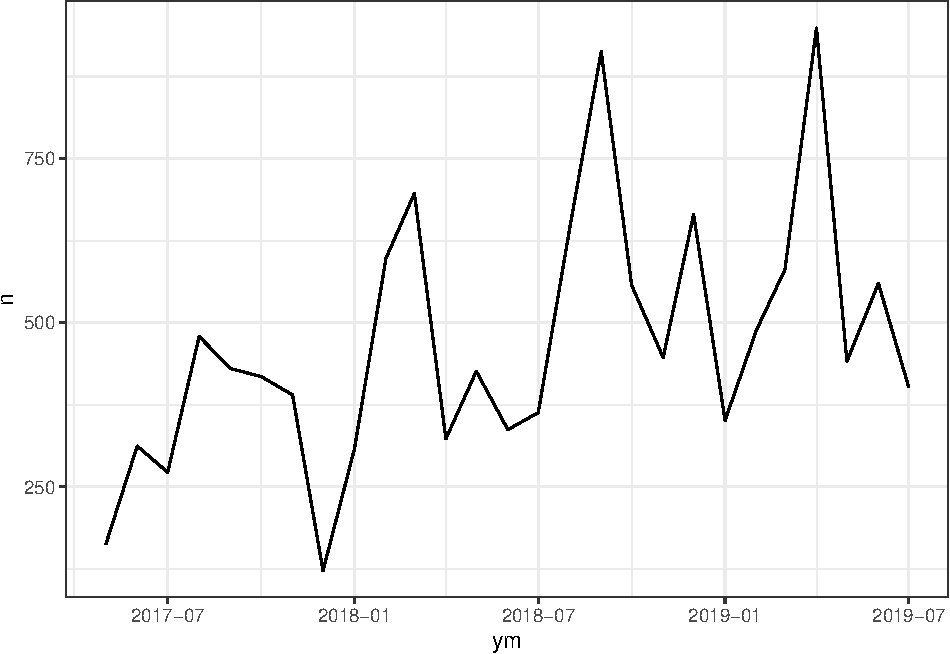
\includegraphics{workshop_topicmodels_files/figure-latex/read-data-1.pdf}

\begin{Shaded}
\begin{Highlighting}[]
\NormalTok{d }\OperatorTok\StringTok{ }
\StringTok{  }\KeywordTok{pull}\NormalTok{(}\StringTok{"wc"}\NormalTok{) }\OperatorTok\StringTok{ }
\StringTok{  }\KeywordTok{summary}\NormalTok{()}
\end{Highlighting}
\end{Shaded}

\begin{verbatim}
##    Min. 1st Qu.  Median    Mean 3rd Qu.    Max. 
##      20      37      60      85     101    2493
\end{verbatim}

\begin{itemize}
\tightlist
\item
  Der Datensatz besteht aus 12,369 Posts.

  \begin{itemize}
  \tightlist
  \item
    Die Variable \texttt{post} enthält den vollen Text des Posts.
  \item
    Die Variable \texttt{author} enthält den Accountnamen, von dem der Post abgegeben wurde.
  \item
    Die Variable \texttt{date} enthält den Tag der Veröffentlichung.
  \item
    Die Variable \texttt{wc} enthält die Zahl der Wörter des Posts.
  \item
    Die Variable \texttt{thread\_title} enthält den Titel des Diskussions-Threads.
  \end{itemize}
\item
  Pro Monat sind zwischen ca. 120 und 1.000 Posts in unserer Stichprobe.
\item
  Typische Posts haben einen Umfang von zwischen 40 und 100 Wörtern (Zur Erinnerung: Sehr kurze Post wurden bereits ausgeschlossen).
\end{itemize}

\hypertarget{aufbereitung-fuxfcr-das-schuxe4tzen-der-topic-models}{%
\section{Aufbereitung für das Schätzen der Topic Models}\label{aufbereitung-fuxfcr-das-schuxe4tzen-der-topic-models}}

\begin{itemize}
\tightlist
\item
  Grundsätzlich gilt: Die verschiedenen Schritte bei der Aufbereitung des Text-Korpus kann die Ergebnisse wesentlich beeinflussen \citep{dennyTextPreprocessingUnsupervised2018, maierApplyingLDATopic2018}. Aber ist es häufig sehr schwierig, theoretisch informierte Entscheidungen zu treffen, da

  \begin{itemize}
  \tightlist
  \item
    unsere Theorien fast immer zu vage sind, um etwas über konkrete, manifeste Eigenschaften der Texte auszusagen
  \item
    es schwer ist, die Folge einer Entscheidung für das technische Schätzen der Modelle und für die substanzielle Interpretation der Ergebnisse vorherzusagen,
  \item
    Entscheidungen \emph{post hoc} auf Basis der Ergebnisse wissenschaftstheoretisch und -praktisch problematisch sein können (\emph{overfitting}, \emph{harking} bzw. \emph{hindsight bias}, etc.).
  \end{itemize}
\item
  In der zugrunde liegenden Studie habe ich versucht, diese Entscheidungen \emph{a priori} zu treffen. Die Entscheidungen basieren aber zugegebenermaßen mehr auf vagen Vermutungen und für mich plausiblen und pragmatischen Überlegungen als auf einer konsistenten Theorie.

  \begin{itemize}
  \tightlist
  \item
    Entfernen von Stoppwörtern: Stoppwörter sind Wörter, die in einer Sprache häufig vorkommen und nicht wesentlich zur Bedeutung eines Texts beitragen. Hier habe ich auf Basis der deutschen Liste im Paket \texttt{\{stopwords\}} und der Worthäufigkeiten im Korpus eine Liste erstellt. Durch das \emph{Pruning} der Dokument-Feature-Matrix (siehe unten) ist die Auswahl der Stoppwörter aber weniger entscheidend, da Wörter, die in sehr vielen Texten des Korpus vorkommen, ohnehin entfernt werden.
  \item
    Zusätzliche Berücksichtigung von Bi- und Tri-Grammen: Ich habe die Kombinationen von zwei oder drei Wörtern, die häufig im Korpus vorkamen, daraufhin gesichtet, ob sie für das Thema Impfen und gesundheitsrelevante Diskussionen zusätzliche Informationen enthalten, die jedes einzelne Wort alleine nicht enthält. Diese Kombinationen wurden als zusätzliche Features aufgenommen.
  \item
    Der Argumentation und den empirischen Ergebnissen von \citet{schofieldComparingApplesApple2016} (deren Aufsatz übrigens einen großartigen Titel hat, großer NLP Nerd Humor) folgend habe ich auf Stemming oder Lemmatisierung verzichtet. In der Tat zeigt sich, dass Wörter mit dem gleichen Wortstamm, wie von \citet{schofieldComparingApplesApple2016} beschrieben, häufig im selben Topic landen.
  \item
    Üblichen Standards \citep[z.B.][]{maierApplyingLDATopic2018} folgend habe ich alle Wörter in Kleinschreibung umgewandelt, Satzzeichen entfernt und URL entfernt. Zahlen habe ich beibehalten, da sie (wie die Ergebnisse auch zeigen) typische Merkmale bestimmter Perspektiven auf das Thema Impfen sind.
  \item
    Da wir auch an der Veränderung der Topic-Häufigkeiten über die Zeit interessiert sind, wird die Variable mit dem Erscheinungstags des Posts in eine numerische Variable umgewandelt. Sie ist so skaliert, dass der aktuellste Post den Wert 0 hat. Diese Variable können wir dann als Prädiktor beim Schätzen des \emph{Structural Topic Model} berücksichtigen.
  \item
    Unter \emph{Pruning} versteht man das Entfernen von Features, die entweder in sehr weniger oder in sehr vielen Dokumenten vorkommen. Dadurch können die Größe des Datensatzes und in der Folge die zum Schätzen der Modelle nötigen Ressourcen wesentlich reduziert werden. Inhaltlich sollte das Entfernen dieser Features wenig ändern: Features, die in sehr vielen Dokumenten vorkommen, tragen nicht zur Differenzierung zwischen den Dokumenten bei. Features, die nur in sehr wenigen Dokumenten vorkommen, tragen nicht zur Definition von Topics bei, da diese durch das regelmäßige \emph{gemeinsame} Vorkommen in Dokumenten identifiziert werden. Siehe ausführlich \citet{maierApplyingLDATopic2018}.
  \end{itemize}
\item
  Die Vorbereitung des Korpus und der Dokument-Feature-Matrix erfolgte mit Funktionen aus \texttt{\{quanteda\}}.

  \begin{itemize}
  \tightlist
  \item
    Mit der Funktion \texttt{corpus()} wird der Datensatz in einen Text-Korpus umgewandelt. In diesem Zuge wird auch die numerische Datums-Variable erstellt. Die Variable mit dem Text des Posts duplizieren wir, damit sie zusätzlich als Meta-Datum für jeden Text gespeichert wird. Das wird später hilfreich sein, wenn wir die Ergebnisse einer Modellschätzung explorieren.
  \item
    \texttt{custom\_stopwords} und \texttt{relevant\_ngrams} zeigen die Stoppwörter und Wortkombinationen, die ausgeschlossen bzw. einbezogen werden. Letztere werden mit der Funktion \texttt{dictionary()} aus \texttt{\{quanteda\}} erstellt.
  \item
    Mit der Funktion \texttt{dfm()} wird der Korpus in eine Dokument-Feature-Matrix umgewandelt. Dabei werden die Standard-Schritte der Textaufbereitung durchgeführt. Sie besteht aus 12,369 Posts in den Zeilen und 41,385 Features in den Spalten. In jeder Zelle ist angegeben, wie häufig ein Feature in einem Dokument vorkommt.
  \item
    Mit der Funktion \texttt{dfm\_trim()} wird das Pruning durchgeführt. Dabei werden alle Features, die in weniger als 0.5\% oder mehr als 99\% der Posts vorkommen, entfernt. Nach dem Pruning enthält die Matrix nur noch 1,150 Features.
  \item
    Zuletzt muss die Matrix in das von \texttt{stm()} benötigte Format konvertiert werden. Dabei werden zwei Posts gelöscht, die nach der Bereinigung kein einziges Feature mehr enthalten. Wichtig für den Bericht der Fallzahl in einer Publikation!
  \end{itemize}
\item
  Am Ende seht ihr eine einfache Beschreibung der häufigsten Features im Korpus als Tabelle und Wordcloud.
\end{itemize}

\begin{Shaded}
\begin{Highlighting}[]
\CommentTok{# Erstellen des Korpus}
\NormalTok{crps =}\StringTok{ }\NormalTok{d }\OperatorTok\StringTok{ }
\StringTok{  }\KeywordTok{mutate}\NormalTok{(}\DataTypeTok{txt =}\NormalTok{ post, }\CommentTok{# Duplizieren des Post-Texts für Meta-Daten}
         \DataTypeTok{date_num =} \KeywordTok{as.numeric}\NormalTok{(postdate) }\OperatorTok{-}\StringTok{ }\KeywordTok{max}\NormalTok{(}\KeywordTok{as.numeric}\NormalTok{(postdate))) }\OperatorTok\StringTok{ }\CommentTok{# Numerische Datumsvariable}
\StringTok{  }\KeywordTok{corpus}\NormalTok{(}\DataTypeTok{text_field =} \StringTok{"post"}\NormalTok{) }\CommentTok{# Erstellen des Korpus}
\NormalTok{crps }\OperatorTok\StringTok{ }
\StringTok{  }\KeywordTok{summary}\NormalTok{(}\DataTypeTok{n =} \DecValTok{1}\NormalTok{)}
\end{Highlighting}
\end{Shaded}

\begin{verbatim}
## Corpus consisting of 12369 documents, showing 1 document:
## 
##   Text Types Tokens Sentences       author   postdate wc thread_title
##  text1    27     29         2 zwerg-bayern 2018-04-06 26  HPV-Impfung
##                                                                                                                                                                                                  txt
##  Wenn Impfungen zu Todesfälle oder starken Nebenwirkungen in einzelnen Fällen führen, spricht dann für Immungschwäche oder schlummernder Krankheit. Ein gesunder Mensch stirbt nicht an der Impfung.
##  date_num
##      -457
\end{verbatim}

\begin{Shaded}
\begin{Highlighting}[]
\CommentTok{# Stoppwörter}
\NormalTok{custom_stopwords =}\StringTok{ }\KeywordTok{c}\NormalTok{(}\StringTok{"ab"}\NormalTok{, }\StringTok{"aber"}\NormalTok{, }\StringTok{"ach"}\NormalTok{, }\StringTok{"all"}\NormalTok{, }\StringTok{"alle"}\NormalTok{, }\StringTok{"allem"}\NormalTok{, }\StringTok{"allen"}\NormalTok{, }\StringTok{"aller"}\NormalTok{, }\StringTok{"alles"}\NormalTok{, }\StringTok{"als"}\NormalTok{, }\StringTok{"also"}\NormalTok{, }\StringTok{"am"}\NormalTok{, }\StringTok{"an"}\NormalTok{, }\StringTok{"andere"}\NormalTok{, }\StringTok{"anderen"}\NormalTok{, }\StringTok{"anderes"}\NormalTok{, }\StringTok{"anders"}\NormalTok{, }\StringTok{"auch"}\NormalTok{, }\StringTok{"auf"}\NormalTok{, }\StringTok{"aufs"}\NormalTok{, }\StringTok{"aus"}\NormalTok{, }\StringTok{"bei"}\NormalTok{, }\StringTok{"beim"}\NormalTok{, }\StringTok{"bin"}\NormalTok{, }\StringTok{"bis"}\NormalTok{, }\StringTok{"bist"}\NormalTok{, }\StringTok{"bzw"}\NormalTok{, }\StringTok{"da"}\NormalTok{, }\StringTok{"dabei"}\NormalTok{, }\StringTok{"dadurch"}\NormalTok{, }\StringTok{"daher"}\NormalTok{, }\StringTok{"dahin"}\NormalTok{, }\StringTok{"damit"}\NormalTok{, }\StringTok{"dann"}\NormalTok{, }\StringTok{"das"}\NormalTok{, }\StringTok{"dass"}\NormalTok{, }\StringTok{"daß"}\NormalTok{, }\StringTok{"dazu"}\NormalTok{, }\StringTok{"dein"}\NormalTok{, }\StringTok{"deine"}\NormalTok{, }\StringTok{"deinem"}\NormalTok{, }\StringTok{"deinen"}\NormalTok{, }\StringTok{"deiner"}\NormalTok{, }\StringTok{"dem"}\NormalTok{, }\StringTok{"den"}\NormalTok{, }\StringTok{"denen"}\NormalTok{, }\StringTok{"denn"}\NormalTok{, }\StringTok{"dennoch"}\NormalTok{, }\StringTok{"der"}\NormalTok{, }\StringTok{"deren"}\NormalTok{, }\StringTok{"des"}\NormalTok{, }\StringTok{"deshalb"}\NormalTok{, }\StringTok{"deswegen"}\NormalTok{, }\StringTok{"dich"}\NormalTok{, }\StringTok{"die"}\NormalTok{, }\StringTok{"dies"}\NormalTok{, }\StringTok{"diese"}\NormalTok{, }\StringTok{"diesem"}\NormalTok{, }\StringTok{"diesen"}\NormalTok{, }\StringTok{"dieser"}\NormalTok{, }\StringTok{"dieses"}\NormalTok{, }\StringTok{"dir"}\NormalTok{, }\StringTok{"doch"}\NormalTok{, }\StringTok{"dort"}\NormalTok{, }\StringTok{"dran"}\NormalTok{, }\StringTok{"drauf"}\NormalTok{, }\StringTok{"drin"}\NormalTok{, }\StringTok{"drüber", "}\NormalTok{du}\StringTok{", "}\NormalTok{durch}\StringTok{", "}\NormalTok{durchaus}\StringTok{", "}\NormalTok{eh}\StringTok{", "}\NormalTok{ein}\StringTok{", "}\NormalTok{eine}\StringTok{", "}\NormalTok{einem}\StringTok{", "}\NormalTok{einen}\StringTok{", "}\NormalTok{einer}\StringTok{", "}\NormalTok{eines}\StringTok{", "}\NormalTok{einige}\StringTok{", "}\NormalTok{einigen}\StringTok{", "}\NormalTok{einiges}\StringTok{", "}\NormalTok{einmal}\StringTok{", "}\NormalTok{er}\StringTok{", "}\NormalTok{es}\StringTok{", "}\NormalTok{etc}\StringTok{", "}\NormalTok{etwas}\StringTok{", "}\NormalTok{euch}\StringTok{", "}\NormalTok{euer}\StringTok{", "}\NormalTok{eure}\StringTok{", "}\NormalTok{euren}\StringTok{", "}\NormalTok{für", }\StringTok{"fürs", "}\NormalTok{gegen}\StringTok{", "}\NormalTok{gehabt}\StringTok{", "}\NormalTok{getan}\StringTok{", "}\NormalTok{gewesen}\StringTok{", "}\NormalTok{geworden}\StringTok{", "}\NormalTok{hab}\StringTok{", "}\NormalTok{habe}\StringTok{", "}\NormalTok{haben}\StringTok{", "}\NormalTok{habt}\StringTok{", "}\NormalTok{halt}\StringTok{", "}\NormalTok{hast}\StringTok{", "}\NormalTok{hat}\StringTok{", "}\NormalTok{hatte}\StringTok{", "}\NormalTok{hätte}\StringTok{", "}\NormalTok{hatten}\StringTok{", "}\NormalTok{hätten}\StringTok{", "}\NormalTok{her}\StringTok{", "}\NormalTok{hier}\StringTok{", "}\NormalTok{hin}\StringTok{", "}\NormalTok{hinter}\StringTok{", "}\NormalTok{ich}\StringTok{", "}\NormalTok{ihm}\StringTok{", "}\NormalTok{ihn}\StringTok{", "}\NormalTok{ihnen}\StringTok{", "}\NormalTok{ihr}\StringTok{", "}\NormalTok{ihre}\StringTok{", "}\NormalTok{ihrem}\StringTok{", "}\NormalTok{ihren}\StringTok{", "}\NormalTok{ihrer}\StringTok{", "}\NormalTok{im}\StringTok{", "}\NormalTok{in}\StringTok{", "}\NormalTok{ins}\StringTok{", "}\NormalTok{is}\StringTok{", "}\NormalTok{ist}\StringTok{", "}\NormalTok{ja}\StringTok{", "}\NormalTok{je}\StringTok{", "}\NormalTok{jede}\StringTok{", "}\NormalTok{jedem}\StringTok{", "}\NormalTok{jeden}\StringTok{", "}\NormalTok{jeder}\StringTok{", "}\NormalTok{jedes}\StringTok{", "}\NormalTok{jetzt}\StringTok{", "}\NormalTok{kann}\StringTok{", "}\NormalTok{kannst}\StringTok{", "}\NormalTok{kein}\StringTok{", "}\NormalTok{keine}\StringTok{", "}\NormalTok{keinem}\StringTok{", "}\NormalTok{keinen}\StringTok{", "}\NormalTok{keiner}\StringTok{", "}\NormalTok{können}\StringTok{", "}\NormalTok{könnt}\StringTok{", "}\NormalTok{konnte}\StringTok{", "}\NormalTok{könnte}\StringTok{", "}\NormalTok{könnten}\StringTok{", "}\NormalTok{mach}\StringTok{", "}\NormalTok{mache}\StringTok{", "}\NormalTok{machen}\StringTok{", "}\NormalTok{machst}\StringTok{", "}\NormalTok{macht}\StringTok{", "}\NormalTok{mal}\StringTok{", "}\NormalTok{man}\StringTok{", "}\NormalTok{manche}\StringTok{", "}\NormalTok{mein}\StringTok{", "}\NormalTok{meine}\StringTok{", "}\NormalTok{meinem}\StringTok{", "}\NormalTok{meinen}\StringTok{", "}\NormalTok{meiner}\StringTok{", "}\NormalTok{meines}\StringTok{", "}\NormalTok{mich}\StringTok{", "}\NormalTok{mir}\StringTok{", "}\NormalTok{mit}\StringTok{", "}\NormalTok{muss}\StringTok{", "}\NormalTok{müssen", }\StringTok{"musst"}\NormalTok{, }\StringTok{"musste"}\NormalTok{, }\StringTok{"müsste", "}\NormalTok{mussten}\StringTok{", "}\NormalTok{na}\StringTok{", "}\NormalTok{nach}\StringTok{", "}\NormalTok{nachdem}\StringTok{", "}\NormalTok{naja}\StringTok{", "}\NormalTok{ne}\StringTok{", "}\NormalTok{nein}\StringTok{", "}\NormalTok{nem}\StringTok{", "}\NormalTok{nen}\StringTok{", "}\NormalTok{ner}\StringTok{", "}\NormalTok{nicht}\StringTok{", "}\NormalTok{nichts}\StringTok{", "}\NormalTok{nix}\StringTok{", "}\NormalTok{noch}\StringTok{", "}\NormalTok{nun}\StringTok{", "}\NormalTok{nur}\StringTok{", "}\NormalTok{ob}\StringTok{", "}\NormalTok{oder}\StringTok{", "}\NormalTok{ohne}\StringTok{", "}\NormalTok{ok}\StringTok{", "}\NormalTok{okay}\StringTok{", "}\NormalTok{raus}\StringTok{", "}\NormalTok{rein}\StringTok{", "}\NormalTok{rum}\StringTok{", "}\NormalTok{schon}\StringTok{", "}\NormalTok{sehr}\StringTok{", "}\NormalTok{sei}\StringTok{", "}\NormalTok{seid}\StringTok{", "}\NormalTok{sein}\StringTok{", "}\NormalTok{seine}\StringTok{", "}\NormalTok{seinem}\StringTok{", "}\NormalTok{seinen}\StringTok{", "}\NormalTok{seiner}\StringTok{", "}\NormalTok{selber}\StringTok{", "}\NormalTok{selbst}\StringTok{", "}\NormalTok{sich}\StringTok{", "}\NormalTok{sie}\StringTok{", "}\NormalTok{sind}\StringTok{", "}\NormalTok{so}\StringTok{", "}\NormalTok{solche}\StringTok{", "}\NormalTok{solchen}\StringTok{", "}\NormalTok{soll}\StringTok{", "}\NormalTok{sollen}\StringTok{", "}\NormalTok{sollte}\StringTok{", "}\NormalTok{sollten}\StringTok{", "}\NormalTok{solltest}\StringTok{", "}\NormalTok{somit}\StringTok{", "}\NormalTok{sondern}\StringTok{", "}\NormalTok{sonst}\StringTok{", "}\NormalTok{sowas}\StringTok{", "}\NormalTok{soweit}\StringTok{", "}\NormalTok{tun}\StringTok{", "}\NormalTok{tut}\StringTok{", "}\NormalTok{über}\StringTok{", "}\NormalTok{um}\StringTok{", "}\NormalTok{und}\StringTok{", "}\NormalTok{uns}\StringTok{", "}\NormalTok{unser}\StringTok{", "}\NormalTok{unsere}\StringTok{", "}\NormalTok{unserem}\StringTok{", "}\NormalTok{unseren}\StringTok{", "}\NormalTok{unserer}\StringTok{", "}\NormalTok{unter}\StringTok{", "}\NormalTok{usw}\StringTok{", "}\NormalTok{viel}\StringTok{", "}\NormalTok{viele}\StringTok{", "}\NormalTok{vielen}\StringTok{", "}\NormalTok{vieles}\StringTok{", "}\NormalTok{vom}\StringTok{", "}\NormalTok{von}\StringTok{", "}\NormalTok{vor}\StringTok{", "}\NormalTok{war}\StringTok{", "}\NormalTok{wäre}\StringTok{", "}\NormalTok{waren}\StringTok{", "}\NormalTok{wären}\StringTok{", "}\NormalTok{wars}\StringTok{", "}\NormalTok{was}\StringTok{", "}\NormalTok{weder}\StringTok{", "}\NormalTok{weg}\StringTok{", "}\NormalTok{wegen}\StringTok{", "}\NormalTok{weil}\StringTok{", "}\NormalTok{weiter}\StringTok{", "}\NormalTok{weitere}\StringTok{", "}\NormalTok{welche}\StringTok{", "}\NormalTok{welchen}\StringTok{", "}\NormalTok{welcher}\StringTok{", "}\NormalTok{welches}\StringTok{", "}\NormalTok{wenn}\StringTok{", "}\NormalTok{wenns}\StringTok{", "}\NormalTok{wer}\StringTok{", "}\NormalTok{werd}\StringTok{", "}\NormalTok{werde}\StringTok{", "}\NormalTok{werden}\StringTok{", "}\NormalTok{wie}\StringTok{", "}\NormalTok{wieder}\StringTok{", "}\NormalTok{wieso}\StringTok{", "}\NormalTok{will}\StringTok{", "}\NormalTok{willst}\StringTok{", "}\NormalTok{wir}\StringTok{", "}\NormalTok{wird}\StringTok{", "}\NormalTok{wirst}\StringTok{", "}\NormalTok{wo}\StringTok{", "}\NormalTok{wobei}\StringTok{", "}\NormalTok{wollen}\StringTok{", "}\NormalTok{wollte}\StringTok{", "}\NormalTok{wollten}\StringTok{", "}\NormalTok{worden}\StringTok{", "}\NormalTok{wurde}\StringTok{", "}\NormalTok{würde", }\StringTok{"wurden"}\NormalTok{, }\StringTok{"würden", "}\NormalTok{z.b}\StringTok{", "}\NormalTok{zb}\StringTok{", "}\NormalTok{zu}\StringTok{", "}\NormalTok{zum}\StringTok{", "}\NormalTok{zur}\StringTok{", "}\NormalTok{zwar}\StringTok{", "}\NormalTok{zwischen}\StringTok{")}

\StringTok{# Kombinationen von Wörtern}
\StringTok{relevant_ngrams = dictionary(list(}
\StringTok{  "}\NormalTok{trotz_impfung}\StringTok{" = "}\NormalTok{trotz impfung}\StringTok{",}
\StringTok{  "}\NormalTok{grippe_impfen}\StringTok{" = "}\NormalTok{grippe impfen}\StringTok{",}
\StringTok{  "}\NormalTok{mmr_impfung}\StringTok{" = "}\NormalTok{mmr impfung}\StringTok{",}
\StringTok{  "}\NormalTok{hepatitis_b}\StringTok{" = "}\NormalTok{hepatitis b}\StringTok{",}
\StringTok{  "}\NormalTok{gut_vertragen}\StringTok{" = "}\NormalTok{gut vertragen}\StringTok{",}
\StringTok{  "}\NormalTok{6fach_impfung}\StringTok{" = "}\NormalTok{6fach impfung}\StringTok{",}
\StringTok{  "}\DecValTok{6}\NormalTok{_fach}\StringTok{" = "}\DecValTok{6}\NormalTok{ fach}\StringTok{",}
\StringTok{  "}\DecValTok{6}\NormalTok{_fach_impfung}\StringTok{" = "}\DecValTok{6}\NormalTok{ fach impfung}\StringTok{",}
\StringTok{  "}\NormalTok{meningokokken_b}\StringTok{" = "}\NormalTok{meningokokken b}\StringTok{",}
\StringTok{  "}\NormalTok{gute_besserung}\StringTok{" = "}\NormalTok{gute besserung}\StringTok{",}
\StringTok{  "}\DecValTok{6}\OperatorTok{-}\NormalTok{fach_impfung}\StringTok{" = "}\DecValTok{6}\OperatorTok{-}\NormalTok{fach impfung}\StringTok{",}
\StringTok{  "}\NormalTok{erhöhte_temperatur}\StringTok{" = "}\NormalTok{erhöhte temperatur}\StringTok{",}
\StringTok{  "}\NormalTok{kein_fieber}\StringTok{" = "}\NormalTok{kein fieber}\StringTok{",}
\StringTok{  "}\NormalTok{kein_problem}\StringTok{" = "}\NormalTok{kein problem}\StringTok{",}
\StringTok{  "}\NormalTok{keine_ahnung}\StringTok{" = "}\NormalTok{keine ahnung}\StringTok{",}
\StringTok{  "}\NormalTok{keine_impfung}\StringTok{" = "}\NormalTok{keine impfung}\StringTok{",}
\StringTok{  "}\NormalTok{nicht_geimpft}\StringTok{" = "}\NormalTok{nicht geimpft}\StringTok{",}
\StringTok{  "}\NormalTok{nicht_impfen}\StringTok{" = "}\NormalTok{nicht impfen}\StringTok{",}
\StringTok{  "}\NormalTok{nicht_zu_impfen}\StringTok{" = "}\NormalTok{nicht zu impfen}\StringTok{",}
\StringTok{  "}\NormalTok{selbst_entscheiden}\StringTok{" = "}\NormalTok{selbst entscheiden}\StringTok{"}
\StringTok{))}

\StringTok{# Erstellen einer Dokument-Feature-Matrix aus dem Korpus}
\StringTok{impf_dfm = crps %>% }
\StringTok{  dfm(stem = FALSE, tolower = TRUE, remove_punct = TRUE,}
\StringTok{      remove = custom_stopwords,}
\StringTok{      remove_url = TRUE, verbose = TRUE,}
\StringTok{      thesaurus = relevant_ngrams)}
\end{Highlighting}
\end{Shaded}

\begin{verbatim}
## Creating a dfm from a corpus input...
\end{verbatim}

\begin{verbatim}
##    ... lowercasing
\end{verbatim}

\begin{verbatim}
##    ... found 12,369 documents, 41,651 features
\end{verbatim}

\begin{verbatim}
##    ... applying a dictionary consisting of 20 keys
##    ... removed 286 features
\end{verbatim}

\begin{Shaded}
\begin{Highlighting}[]
\NormalTok{impf_dfm}
\end{Highlighting}
\end{Shaded}

\begin{verbatim}
## Document-feature matrix of: 12,369 documents, 41,385 features (99.9% sparse) and 6 docvars.
##        features
## docs    TROTZ_IMPFUNG GRIPPE_IMPFEN MMR_IMPFUNG HEPATITIS_B GUT_VERTRAGEN
##   text1             0             0           0           0             0
##   text2             0             0           0           0             0
##   text3             0             0           0           0             0
##   text4             1             0           0           0             0
##   text5             0             0           0           0             0
##   text6             0             0           0           0             0
##        features
## docs    6FACH_IMPFUNG 6_FACH 6_FACH_IMPFUNG MENINGOKOKKEN_B GUTE_BESSERUNG
##   text1             0      0              0               0              0
##   text2             0      0              0               0              0
##   text3             0      0              0               0              0
##   text4             1      0              0               0              0
##   text5             0      0              0               0              0
##   text6             0      0              0               0              0
## [ reached max_ndoc ... 12,363 more documents, reached max_nfeat ... 41,375 more features ]
\end{verbatim}

\begin{Shaded}
\begin{Highlighting}[]
\CommentTok{# Pruning}
\NormalTok{impf_dfm =}\StringTok{ }\NormalTok{impf_dfm }\OperatorTok
\StringTok{  }\KeywordTok{dfm_trim}\NormalTok{(}\DataTypeTok{max_docfreq =} \FloatTok{0.99}\NormalTok{, }\DataTypeTok{min_docfreq =} \FloatTok{0.005}\NormalTok{, }\DataTypeTok{docfreq_type =} \StringTok{"prop"}\NormalTok{)}
\NormalTok{impf_dfm}
\end{Highlighting}
\end{Shaded}

\begin{verbatim}
## Document-feature matrix of: 12,369 documents, 1,150 features (98.2% sparse) and 6 docvars.
##        features
## docs    TROTZ_IMPFUNG GRIPPE_IMPFEN MMR_IMPFUNG GUT_VERTRAGEN 6_FACH
##   text1             0             0           0             0      0
##   text2             0             0           0             0      0
##   text3             0             0           0             0      0
##   text4             1             0           0             0      0
##   text5             0             0           0             0      0
##   text6             0             0           0             0      0
##        features
## docs    MENINGOKOKKEN_B GUTE_BESSERUNG ERHÖHTE_TEMPERATUR KEIN_FIEBER
##   text1               0              0                  0           0
##   text2               0              0                  0           0
##   text3               0              0                  0           0
##   text4               0              0                  0           0
##   text5               0              0                  0           0
##   text6               0              0                  0           0
##        features
## docs    KEIN_PROBLEM
##   text1            0
##   text2            0
##   text3            0
##   text4            0
##   text5            0
##   text6            0
## [ reached max_ndoc ... 12,363 more documents, reached max_nfeat ... 1,140 more features ]
\end{verbatim}

\begin{Shaded}
\begin{Highlighting}[]
\CommentTok{# Überblick: Die häufigsten Features im Korpus}
\NormalTok{impf_dfm }\OperatorTok\StringTok{ }
\StringTok{  }\KeywordTok{colSums}\NormalTok{() }\OperatorTok\StringTok{ }
\StringTok{  }\KeywordTok{enframe}\NormalTok{() }\OperatorTok\StringTok{ }
\StringTok{  }\KeywordTok{arrange}\NormalTok{(}\KeywordTok{desc}\NormalTok{(value)) }\OperatorTok\StringTok{ }
\StringTok{  }\KeywordTok{slice}\NormalTok{(}\DecValTok{1}\OperatorTok{:}\DecValTok{20}\NormalTok{) }\OperatorTok\StringTok{ }
\StringTok{  }\KeywordTok{kable}\NormalTok{()}
\end{Highlighting}
\end{Shaded}

\begin{tabular}{l|r}
\hline
name & value\\
\hline
impfung & 4519\\
\hline
impfen & 4356\\
\hline
kind & 3690\\
\hline
lassen & 3257\\
\hline
immer & 2705\\
\hline
mehr & 2594\\
\hline
kinder & 2503\\
\hline
gibt & 2184\\
\hline
geimpft & 2176\\
\hline
impfungen & 2174\\
\hline
gut & 2115\\
\hline
hallo & 1898\\
\hline
einfach & 1767\\
\hline
lg & 1720\\
\hline
2 & 1704\\
\hline
bekommen & 1585\\
\hline
ganz & 1584\\
\hline
erst & 1558\\
\hline
geht & 1492\\
\hline
arzt & 1411\\
\hline
\end{tabular}

\begin{Shaded}
\begin{Highlighting}[]
\CommentTok{# als (beliebte, wenn auch nur mittel informative) Wordcloud}
\NormalTok{impf_dfm }\OperatorTok\StringTok{ }
\StringTok{  }\KeywordTok{textplot_wordcloud}\NormalTok{()}
\end{Highlighting}
\end{Shaded}

\begin{verbatim}
## Warning in graphics::strwidth(word[i], cex = size[i]): Konvertierungsfehler für
## '😊' in 'mbcsToSbcs': Punkt ersetzt <f0>
\end{verbatim}

\begin{verbatim}
## Warning in graphics::strwidth(word[i], cex = size[i]): Konvertierungsfehler für
## '😊' in 'mbcsToSbcs': Punkt ersetzt <9f>
\end{verbatim}

\begin{verbatim}
## Warning in graphics::strwidth(word[i], cex = size[i]): Konvertierungsfehler für
## '😊' in 'mbcsToSbcs': Punkt ersetzt <98>
\end{verbatim}

\begin{verbatim}
## Warning in graphics::strwidth(word[i], cex = size[i]): Konvertierungsfehler für
## '😊' in 'mbcsToSbcs': Punkt ersetzt <8a>
\end{verbatim}

\begin{verbatim}
## Warning in text.default(x1, y1, word[i], cex = (1 + adjust) * size[i], offset =
## 0, : Konvertierungsfehler für '😊' in 'mbcsToSbcs': Punkt ersetzt <f0>
\end{verbatim}

\begin{verbatim}
## Warning in text.default(x1, y1, word[i], cex = (1 + adjust) * size[i], offset =
## 0, : Konvertierungsfehler für '😊' in 'mbcsToSbcs': Punkt ersetzt <9f>
\end{verbatim}

\begin{verbatim}
## Warning in text.default(x1, y1, word[i], cex = (1 + adjust) * size[i], offset =
## 0, : Konvertierungsfehler für '😊' in 'mbcsToSbcs': Punkt ersetzt <98>
\end{verbatim}

\begin{verbatim}
## Warning in text.default(x1, y1, word[i], cex = (1 + adjust) * size[i], offset =
## 0, : Konvertierungsfehler für '😊' in 'mbcsToSbcs': Punkt ersetzt <8a>
\end{verbatim}

\begin{verbatim}
## Warning in text.default(x1, y1, word[i], cex = (1 + adjust) * size[i], offset =
## 0, : Fontmetrik ist für das Unicode-Zeichen U+1f60a unbekannt
\end{verbatim}

\begin{verbatim}
## Warning in graphics::strwidth(word[i], cex = size[i]): Konvertierungsfehler für
## '😂' in 'mbcsToSbcs': Punkt ersetzt <f0>
\end{verbatim}

\begin{verbatim}
## Warning in graphics::strwidth(word[i], cex = size[i]): Konvertierungsfehler für
## '😂' in 'mbcsToSbcs': Punkt ersetzt <9f>
\end{verbatim}

\begin{verbatim}
## Warning in graphics::strwidth(word[i], cex = size[i]): Konvertierungsfehler für
## '😂' in 'mbcsToSbcs': Punkt ersetzt <98>
\end{verbatim}

\begin{verbatim}
## Warning in graphics::strwidth(word[i], cex = size[i]): Konvertierungsfehler für
## '😂' in 'mbcsToSbcs': Punkt ersetzt <82>
\end{verbatim}

\begin{verbatim}
## Warning in text.default(x1, y1, word[i], cex = (1 + adjust) * size[i], offset =
## 0, : Konvertierungsfehler für '😂' in 'mbcsToSbcs': Punkt ersetzt <f0>
\end{verbatim}

\begin{verbatim}
## Warning in text.default(x1, y1, word[i], cex = (1 + adjust) * size[i], offset =
## 0, : Konvertierungsfehler für '😂' in 'mbcsToSbcs': Punkt ersetzt <9f>
\end{verbatim}

\begin{verbatim}
## Warning in text.default(x1, y1, word[i], cex = (1 + adjust) * size[i], offset =
## 0, : Konvertierungsfehler für '😂' in 'mbcsToSbcs': Punkt ersetzt <98>
\end{verbatim}

\begin{verbatim}
## Warning in text.default(x1, y1, word[i], cex = (1 + adjust) * size[i], offset =
## 0, : Konvertierungsfehler für '😂' in 'mbcsToSbcs': Punkt ersetzt <82>
\end{verbatim}

\begin{verbatim}
## Warning in text.default(x1, y1, word[i], cex = (1 + adjust) * size[i], offset =
## 0, : Fontmetrik ist für das Unicode-Zeichen U+1f602 unbekannt
\end{verbatim}

\begin{verbatim}
## Warning in graphics::strwidth(word[i], cex = size[i]): Konvertierungsfehler für
## '😉' in 'mbcsToSbcs': Punkt ersetzt <f0>
\end{verbatim}

\begin{verbatim}
## Warning in graphics::strwidth(word[i], cex = size[i]): Konvertierungsfehler für
## '😉' in 'mbcsToSbcs': Punkt ersetzt <9f>
\end{verbatim}

\begin{verbatim}
## Warning in graphics::strwidth(word[i], cex = size[i]): Konvertierungsfehler für
## '😉' in 'mbcsToSbcs': Punkt ersetzt <98>
\end{verbatim}

\begin{verbatim}
## Warning in graphics::strwidth(word[i], cex = size[i]): Konvertierungsfehler für
## '😉' in 'mbcsToSbcs': Punkt ersetzt <89>
\end{verbatim}

\begin{verbatim}
## Warning in text.default(x1, y1, word[i], cex = (1 + adjust) * size[i], offset =
## 0, : Konvertierungsfehler für '😉' in 'mbcsToSbcs': Punkt ersetzt <f0>
\end{verbatim}

\begin{verbatim}
## Warning in text.default(x1, y1, word[i], cex = (1 + adjust) * size[i], offset =
## 0, : Konvertierungsfehler für '😉' in 'mbcsToSbcs': Punkt ersetzt <9f>
\end{verbatim}

\begin{verbatim}
## Warning in text.default(x1, y1, word[i], cex = (1 + adjust) * size[i], offset =
## 0, : Konvertierungsfehler für '😉' in 'mbcsToSbcs': Punkt ersetzt <98>
\end{verbatim}

\begin{verbatim}
## Warning in text.default(x1, y1, word[i], cex = (1 + adjust) * size[i], offset =
## 0, : Konvertierungsfehler für '😉' in 'mbcsToSbcs': Punkt ersetzt <89>
\end{verbatim}

\begin{verbatim}
## Warning in text.default(x1, y1, word[i], cex = (1 + adjust) * size[i], offset =
## 0, : Fontmetrik ist für das Unicode-Zeichen U+1f609 unbekannt
\end{verbatim}

\begin{verbatim}
## Warning in graphics::strwidth(word[i], cex = size[i]): Konvertierungsfehler für
## '🙈' in 'mbcsToSbcs': Punkt ersetzt <f0>
\end{verbatim}

\begin{verbatim}
## Warning in graphics::strwidth(word[i], cex = size[i]): Konvertierungsfehler für
## '🙈' in 'mbcsToSbcs': Punkt ersetzt <9f>
\end{verbatim}

\begin{verbatim}
## Warning in graphics::strwidth(word[i], cex = size[i]): Konvertierungsfehler für
## '🙈' in 'mbcsToSbcs': Punkt ersetzt <99>
\end{verbatim}

\begin{verbatim}
## Warning in graphics::strwidth(word[i], cex = size[i]): Konvertierungsfehler für
## '🙈' in 'mbcsToSbcs': Punkt ersetzt <88>
\end{verbatim}

\begin{verbatim}
## Warning in text.default(x1, y1, word[i], cex = (1 + adjust) * size[i], offset =
## 0, : Konvertierungsfehler für '🙈' in 'mbcsToSbcs': Punkt ersetzt <f0>
\end{verbatim}

\begin{verbatim}
## Warning in text.default(x1, y1, word[i], cex = (1 + adjust) * size[i], offset =
## 0, : Konvertierungsfehler für '🙈' in 'mbcsToSbcs': Punkt ersetzt <9f>
\end{verbatim}

\begin{verbatim}
## Warning in text.default(x1, y1, word[i], cex = (1 + adjust) * size[i], offset =
## 0, : Konvertierungsfehler für '🙈' in 'mbcsToSbcs': Punkt ersetzt <99>
\end{verbatim}

\begin{verbatim}
## Warning in text.default(x1, y1, word[i], cex = (1 + adjust) * size[i], offset =
## 0, : Konvertierungsfehler für '🙈' in 'mbcsToSbcs': Punkt ersetzt <88>
\end{verbatim}

\begin{verbatim}
## Warning in text.default(x1, y1, word[i], cex = (1 + adjust) * size[i], offset =
## 0, : Fontmetrik ist für das Unicode-Zeichen U+1f648 unbekannt
\end{verbatim}

\begin{verbatim}
## Warning in graphics::strwidth(word[i], cex = size[i]): Konvertierungsfehler für
## '😅' in 'mbcsToSbcs': Punkt ersetzt <f0>
\end{verbatim}

\begin{verbatim}
## Warning in graphics::strwidth(word[i], cex = size[i]): Konvertierungsfehler für
## '😅' in 'mbcsToSbcs': Punkt ersetzt <9f>
\end{verbatim}

\begin{verbatim}
## Warning in graphics::strwidth(word[i], cex = size[i]): Konvertierungsfehler für
## '😅' in 'mbcsToSbcs': Punkt ersetzt <98>
\end{verbatim}

\begin{verbatim}
## Warning in graphics::strwidth(word[i], cex = size[i]): Konvertierungsfehler für
## '😅' in 'mbcsToSbcs': Punkt ersetzt <85>
\end{verbatim}

\begin{verbatim}
## Warning in text.default(x1, y1, word[i], cex = (1 + adjust) * size[i], offset =
## 0, : Konvertierungsfehler für '😅' in 'mbcsToSbcs': Punkt ersetzt <f0>
\end{verbatim}

\begin{verbatim}
## Warning in text.default(x1, y1, word[i], cex = (1 + adjust) * size[i], offset =
## 0, : Konvertierungsfehler für '😅' in 'mbcsToSbcs': Punkt ersetzt <9f>
\end{verbatim}

\begin{verbatim}
## Warning in text.default(x1, y1, word[i], cex = (1 + adjust) * size[i], offset =
## 0, : Konvertierungsfehler für '😅' in 'mbcsToSbcs': Punkt ersetzt <98>
\end{verbatim}

\begin{verbatim}
## Warning in text.default(x1, y1, word[i], cex = (1 + adjust) * size[i], offset =
## 0, : Konvertierungsfehler für '😅' in 'mbcsToSbcs': Punkt ersetzt <85>
\end{verbatim}

\begin{verbatim}
## Warning in text.default(x1, y1, word[i], cex = (1 + adjust) * size[i], offset =
## 0, : Fontmetrik ist für das Unicode-Zeichen U+1f605 unbekannt
\end{verbatim}

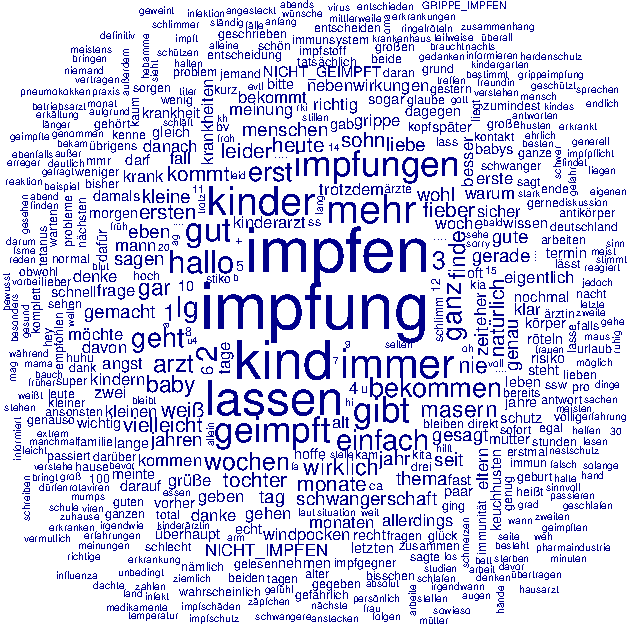
\includegraphics{workshop_topicmodels_files/figure-latex/prepare-data-1.pdf}

\begin{Shaded}
\begin{Highlighting}[]
\CommentTok{# Umwandeln der dfm in das Format für stm}
\NormalTok{impf_stm =}\StringTok{ }\NormalTok{impf_dfm }\OperatorTok\StringTok{ }
\StringTok{  }\NormalTok{quanteda}\OperatorTok{::}\KeywordTok{convert}\NormalTok{(}\DataTypeTok{to =} \StringTok{"stm"}\NormalTok{)}
\end{Highlighting}
\end{Shaded}

\begin{verbatim}
## Warning in dfm2stm(x, docvars, omit_empty = TRUE): Dropped empty document(s):
## text12225, text12271
\end{verbatim}

\hypertarget{modellspezifikation-modellvergleich-und-modellauswahl}{%
\chapter{Modellspezifikation, Modellvergleich und Modellauswahl}\label{modellspezifikation-modellvergleich-und-modellauswahl}}

\hypertarget{modellspezifikation}{%
\section{Modellspezifikation}\label{modellspezifikation}}

\begin{itemize}
\item
  Die Funktion \texttt{stm()} aus dem gleichnamigen Paket bietet zahlreiche Möglichkeiten, Details der Modellspezifikation und -schätzung anzupassen. Wir beschränken uns im Folgenden auf drei wesentliche Einstellungen:

  \begin{itemize}
  \tightlist
  \item
    \texttt{K}: Die Zahl der Topics.
  \item
    \texttt{prevalence}: Eine Formel zur Vorhersage der Topic-Prävalenzen
  \item
    \texttt{init.type}: Wie soll der Startpunkt für die Modellschätzung gewählt werden?
  \end{itemize}
\item
  Zu weiteren Details siehe für einen Überblick \texttt{?stm} und \citet{robertsStmPackageStructural2019} für eine ausführliche Erläuterung.
\item
  Eine Modell-Spezifikation könnte z.B. so aussehen:
\end{itemize}

\begin{Shaded}
\begin{Highlighting}[]
\NormalTok{modelfit =}\StringTok{ }\KeywordTok{stm}\NormalTok{(}\DataTypeTok{documents =}\NormalTok{ impf_stm}\OperatorTok{$}\NormalTok{documents,}
               \DataTypeTok{vocab =}\NormalTok{ impf_stm}\OperatorTok{$}\NormalTok{vocab,}
               \DataTypeTok{data =}\NormalTok{ impf_stm}\OperatorTok{$}\NormalTok{meta, }
               \DataTypeTok{K =} \DecValTok{10}\NormalTok{, }
               \DataTypeTok{prevalence =} \OperatorTok{~}\KeywordTok{s}\NormalTok{(date_num), }
               \DataTypeTok{init.type =} \StringTok{"Spectral"}\NormalTok{)}
\end{Highlighting}
\end{Shaded}

\begin{itemize}
\tightlist
\item
  Mit den ersten drei Inputs übergeben wir die Daten aus der im letzten Abschnitt erstellten Dokument-Feature-Matrix.
\item
  Mit \texttt{K} geben wir an, wie viele Themen es geben soll. Mit dieser Syntax würde ein Modell mit \(k = 10\) Themen geschätzt. Wie wir bei der Wahl eines geeigneten \(k\) vorgehen können, ist Thema des folgenden Unterabschnitts.
\item
  Mit der Formel zu \texttt{prevalence} geben wir an, welche Dokument-Variablen mit dem Auftreten der Topics zusammenhängen.

  \begin{itemize}
  \tightlist
  \item
    In der Formel wird die abhängige Variable vor der Tilde (\textasciitilde) frei gelassen. Es wird immer der Zusammenhang mit dem Auftreten von allen \(k\) Topics geschätzt. In diesem Beispiel schätzen wir, wie sich das Auftreten der Topics über den Untersuchungszeitraum hinweg verändert. Details zum Schätzen von Zusammenhängen mit Kovariaten folgen später in diesem Workshop.
  \item
    Mit \texttt{init.type} wird angegeben, wie \texttt{stm()} die Ausgangswerte für die Modellschätzung bestimmen soll. Die Default-Einstellung ist ``Spectral''. Ich empfehle diese Einstellung aus folgenden Gründen:

    \begin{itemize}
    \tightlist
    \item
      Sie ist deterministisch, d.h., sie führt gegeben derselben Daten und desselben Modells immer zu derselben Lösung. So wird die Reproduzierbarkeit sichergestellt.
    \item
      Sie ist effizient, d.h., dass von diesem Startpunkt aus relativ schnell die finale Lösung gefunden wird.
    \item
      Wenn eine andere Einstellung für die Ausgangswerte gewählt wird, müssen mehrere Schätzungen für eine Spezifikation durchgeführt werden. Nur so kann geprüft werden, ob die Ausgangswerte das Ergebnis beeinflussen.
    \end{itemize}
  \end{itemize}
\item
  Allgemein muss beachtet werden, dass die Schätzung eines Structural Topic Model mit \texttt{stm()} trotz der Effizienz der Implementierung sehr rechenintensiv ist. Die Schätzung des oben beschriebenen Modells dauert auf meinem recht leistungsfähigen Notebook bereits ca. eine Minute. Es empfiehlt sich daher, die Modelle immer in neue Objekte zu speichern und diese ggf. direkt auf der Festplatte zu sichern. Um die Berechnungszeiten in diesem Workshop kurz zu halten, stelle ich die Ergebnisse der Modellschätzungen über das LMS zur Verfügung. Wenn ihr diese herunterladet und in den Ordner ``data'' kopiert, muss das Modell nicht neu geschätzt werden.
\end{itemize}

\hypertarget{modellvergleich}{%
\section{Modellvergleich}\label{modellvergleich}}

\hypertarget{allgemeines-vorgehen}{%
\subsection{Allgemeines Vorgehen}\label{allgemeines-vorgehen}}

\begin{itemize}
\tightlist
\item
  Eine zentrale Frage ist die Wahl eines geeigneten \(k\), also der Zahl von Topics, die in den Dokumenten identifiziert werden sollen. Wichtig ist zuerst die Feststellung, dass es in der angewandten Analyse kein \emph{per se} richtiges oder falsches \(k\) gibt.
\item
  Wie viele Topics nützlich sind, hängt von Umfang von Zusammensetzung des Materials und vom substantiellen Forschungsinteresse ab.
\item
  Um ein geeignetes \(k\) zu finden, gehen wir in der Regel modellvergleichend vor. Wir schätzen Modelle mit unterschiedlich vielen Topics und prüfen dann, welche Modelle besser zu den Daten und zum Forschungsinteresse passen.
\item
  Hinweise für einen allgemeinen Ausgangspunkt, in welchem Bereich nützliche \(k\) zu finden sein könnten, liefert die Paket-Hilfe:
\end{itemize}

\begin{quote}
The most important user input in parametric topic models is the number of topics. There is no right answer to the appropriate number of topics. More topics will give more fine-grained representations of the data at the potential cost of being less precisely estimated. {[}\ldots{]} For short corpora focused on very specific subject matter (such as survey experiments) 3-10 topics is a useful starting range. For small corpora (a few hundred to a few thousand) 5-50 topics is a good place to start. Beyond these rough guidelines it is application specific. Previous applications in political science with medium sized corpora (10k to 100k documents) have found 60-100 topics to work well. For larger corpora 100 topics is a useful default size. Of course, your mileage may vary. --- ?stm
\end{quote}

\begin{itemize}
\tightlist
\item
  Hier werden zwei wichtige Kriterien, die unser Nachdenken über die Spannweite von zu Berücksichtigten \(k\) leiten können, deutlich:

  \begin{itemize}
  \tightlist
  \item
    Quantität des Materials: Je mehr Dokumente, desto mehr Topics.
  \item
    Varianz im Inhalt: Je mehr inhaltliche Varianz, desto mehr Topics (an einem Beispiel: für 10k Nachrichtenbeiträge aus dem Wirtschaftsteil brauchen wir weniger Topics als für 10k Nachrichtenbeiträge, die aus allen Ressorts kommen).
  \end{itemize}
\item
  Im vorliegenden Fall haben wir einen kleinen bis mittleren Korpus (ca. 13k Dokumente, die größtenteils recht kurz sind). Wir können von einer mittleren inhaltlichen Varianz ausgehen. Einerseits haben wir Posts bewusst danach ausgewählt, dass sie sich mit dem Thema Impfen beschäftigen, was die Varianz einschränkt. Andererseits wissen wir, dass in Online-Foren die verschiedensten Perspektiven auf dieses Thema vorkommen können, was für Varianz sorgt.
\item
  Wir gehen im Folgenden in mehreren Schritten vor:

  \begin{enumerate}
  \def\labelenumi{\arabic{enumi})}
  \tightlist
  \item
    Um eine allgemeine Orientierung zu erhalten, in welcher Range Modelle zu finden sind, die gut zu den Daten passen, schätzen wir 10 Modelle von \(k = 10\) bis \(k = 100\) mit einem Abstand von jeweils 10 Topics. Diese Modelle vergleichen wir anhand von einigen statistischen Maßen, um die Zahl der Kandidatenmodelle einzuschränken.
  \item
    Wir interpretieren die besten Modelle substantiell und entscheiden, welche Topic-Anzahl für das Forschungsinteresse hilfreicher scheint.
  \item
    Wir schätzen weitere Modelle basierend auf den Ergebnissen aus 2) mit kleineren Abständen zwischen den \(k\). Wir prüfen, wie sich die Topics verändern. Zudem achten wir darauf, ob bei Modellen mit größeren \(k\) interessante Topics hinzukommen oder ob sich mehr Ambivalenzen zeigen.
  \item
    Wir entscheiden uns für ein Modell.
  \end{enumerate}
\item
  Da das Schätzen der Modelle recht lange dauert, parallelisieren wir die Berechnung. Dazu nutze ich das Paket \texttt{furrr}. Es sei an dieser Stelle darauf hingewiesen, dass das Paket vor allem unter Windows mit RStudio für Probleme sorgen kann. Es ist daher empfehlenswert, das Skript zum Schätzen und Speichern der Modelle in der Konsole oder im Terminal auszuführen. Noch schneller geht es für diesen Workshop, die bereits geschätzten Modelle aus dem LMS zu laden.
\end{itemize}

\hypertarget{quantitativer-vergleich-der-ersten-modelle}{%
\subsection{Quantitativer Vergleich der ersten Modelle}\label{quantitativer-vergleich-der-ersten-modelle}}

\begin{Shaded}
\begin{Highlighting}[]
\CommentTok{# 1) Modelle mit K = 10, ..., K = 100}
\CommentTok{# Modelle schätzen bzw. laden}
\ControlFlowTok{if}\NormalTok{ (}\KeywordTok{file.exists}\NormalTok{(}\StringTok{"R/data/models10_100.rds"}\NormalTok{)) \{}
\CommentTok{# Schneller: Modelle aus LMS laden}
\NormalTok{  many_models =}\StringTok{ }\KeywordTok{read_rds}\NormalTok{(}\StringTok{"R/data/models10_100.rds"}\NormalTok{)}
\NormalTok{\} }\ControlFlowTok{else}\NormalTok{ \{}
\CommentTok{# Vorsicht: Schätzen dauert auf meinem MacBook Pro 2020 i9 32 GB RAM 10 Minuten}
\NormalTok{  Ks =}\StringTok{ }\KeywordTok{seq}\NormalTok{(}\DecValTok{10}\NormalTok{, }\DecValTok{100}\NormalTok{, }\DataTypeTok{by =} \DecValTok{10}\NormalTok{)}
  \KeywordTok{tic}\NormalTok{()}
  \KeywordTok{plan}\NormalTok{(}\KeywordTok{multiprocess}\NormalTok{(}\DataTypeTok{workers =} \DecValTok{10}\NormalTok{))}
\NormalTok{  many_models =}\StringTok{ }\KeywordTok{tibble}\NormalTok{(}\DataTypeTok{K =}\NormalTok{ Ks) }\OperatorTok
\StringTok{    }\KeywordTok{mutate}\NormalTok{(}\DataTypeTok{topic_model =} \KeywordTok{future_map}\NormalTok{(K, }\OperatorTok{~}\KeywordTok{stm}\NormalTok{(}\DataTypeTok{documents =}\NormalTok{ impf_stm}\OperatorTok{$}\NormalTok{documents, }
                                            \DataTypeTok{vocab =}\NormalTok{ impf_stm}\OperatorTok{$}\NormalTok{vocab,}
                                            \DataTypeTok{data =}\NormalTok{ impf_stm}\OperatorTok{$}\NormalTok{meta,}
                                            \DataTypeTok{init.type =} \StringTok{"Spectral"}\NormalTok{,}
                                            \DataTypeTok{K =}\NormalTok{ ., }\DataTypeTok{verbose =} \OtherTok{FALSE}\NormalTok{),}
                                    \DataTypeTok{.progress =} \OtherTok{TRUE}\NormalTok{))}
  \KeywordTok{plan}\NormalTok{(sequential)}
  \KeywordTok{toc}\NormalTok{()}
  \KeywordTok{saveRDS}\NormalTok{(many_models, }\StringTok{"R/data/models10_100.rds"}\NormalTok{)  }
\NormalTok{\}}

\CommentTok{# Quantitative Indikatoren der Modellqualität berechnen}
\CommentTok{# Inspired by https://juliasilge.com/blog/evaluating-stm/}
\ControlFlowTok{if}\NormalTok{ (}\KeywordTok{file.exists}\NormalTok{(}\StringTok{"R/data/eval10_100.rds"}\NormalTok{)) \{}
  \CommentTok{# Schneller: Modellevaluation aus LMS laden}
\NormalTok{  model_eval =}\StringTok{ }\KeywordTok{read_rds}\NormalTok{(}\StringTok{"R/data/eval10_100.rds"}\NormalTok{)}
\NormalTok{\} }\ControlFlowTok{else}\NormalTok{ \{}
  \CommentTok{# Evaluation dauert auf meinem MacBook Pro 2020 i9 32 GB RAM 24 Sekunden}
  \KeywordTok{tic}\NormalTok{()}
\NormalTok{  heldout =}\StringTok{ }\KeywordTok{make.heldout}\NormalTok{(}\DataTypeTok{documents =}\NormalTok{ impf_stm}\OperatorTok{$}\NormalTok{documents, }\DataTypeTok{vocab =}\NormalTok{ impf_stm}\OperatorTok{$}\NormalTok{vocab)}
  \KeywordTok{plan}\NormalTok{(}\KeywordTok{multiprocess}\NormalTok{(}\DataTypeTok{workers =} \DecValTok{10}\NormalTok{))}
\NormalTok{  model_eval =}\StringTok{ }\NormalTok{many_models }\OperatorTok\StringTok{ }
\StringTok{    }\KeywordTok{mutate}\NormalTok{(}\DataTypeTok{exclusivity =} \KeywordTok{future_map}\NormalTok{(topic_model, exclusivity),}
           \DataTypeTok{semantic_coherence =} \KeywordTok{future_map}\NormalTok{(topic_model, semanticCoherence, impf_stm}\OperatorTok{$}\NormalTok{documents),}
           \DataTypeTok{eval_heldout =} \KeywordTok{future_map}\NormalTok{(topic_model, eval.heldout, heldout}\OperatorTok{$}\NormalTok{missing),}
           \DataTypeTok{residual =} \KeywordTok{future_map}\NormalTok{(topic_model, checkResiduals, impf_stm}\OperatorTok{$}\NormalTok{documents),}
           \DataTypeTok{residuals =} \KeywordTok{future_map_dbl}\NormalTok{(residual, }\StringTok{"dispersion"}\NormalTok{),}
           \DataTypeTok{held_out_likelihood =} \KeywordTok{future_map_dbl}\NormalTok{(eval_heldout, }\StringTok{"expected.heldout"}\NormalTok{)) }\OperatorTok\StringTok{ }
\StringTok{    }\KeywordTok{select}\NormalTok{(}\OperatorTok{-}\NormalTok{topic_model)}
  \KeywordTok{plan}\NormalTok{(sequential)}
  \KeywordTok{toc}\NormalTok{()}
  \KeywordTok{saveRDS}\NormalTok{(model_eval, }\StringTok{"R/data/eval10_100.rds"}\NormalTok{)  }
\NormalTok{\}}

\CommentTok{# Exklusivität und Semantische Kohärenz (Mean, Median)}
\NormalTok{model_eval }\OperatorTok\StringTok{ }
\StringTok{  }\KeywordTok{select}\NormalTok{(K, }\DataTypeTok{Exclusivity =}\NormalTok{ exclusivity, }\DataTypeTok{Coherence =}\NormalTok{ semantic_coherence) }\OperatorTok\StringTok{ }
\StringTok{  }\KeywordTok{mutate_at}\NormalTok{(}\OperatorTok{-}\DecValTok{1}\NormalTok{, }\DataTypeTok{.funs =} \KeywordTok{list}\NormalTok{(}\DataTypeTok{Mean =} \OperatorTok{~}\KeywordTok{map_dbl}\NormalTok{(.x, mean), }\DataTypeTok{Median =} \OperatorTok{~}\KeywordTok{map_dbl}\NormalTok{(.x, median))) }\OperatorTok\StringTok{ }
\StringTok{  }\KeywordTok{select_if}\NormalTok{(}\KeywordTok{negate}\NormalTok{(is.list)) }\OperatorTok\StringTok{ }
\StringTok{  }\KeywordTok{gather}\NormalTok{(metric, value, }\OperatorTok{-}\NormalTok{K) }\OperatorTok\StringTok{ }
\StringTok{  }\KeywordTok{separate}\NormalTok{(metric, }\KeywordTok{c}\NormalTok{(}\StringTok{"measure"}\NormalTok{, }\StringTok{"metric"}\NormalTok{), }\StringTok{"_"}\NormalTok{) }\OperatorTok\StringTok{ }
\StringTok{  }\KeywordTok{spread}\NormalTok{(measure, value) }\OperatorTok\StringTok{ }
\StringTok{  }\KeywordTok{ggplot}\NormalTok{(}\KeywordTok{aes}\NormalTok{(Coherence, Exclusivity, }\DataTypeTok{label =}\NormalTok{ K)) }\OperatorTok{+}\StringTok{ }\KeywordTok{geom_text}\NormalTok{() }\OperatorTok{+}\StringTok{ }\KeywordTok{facet_wrap}\NormalTok{(}\StringTok{"metric"}\NormalTok{)}
\end{Highlighting}
\end{Shaded}

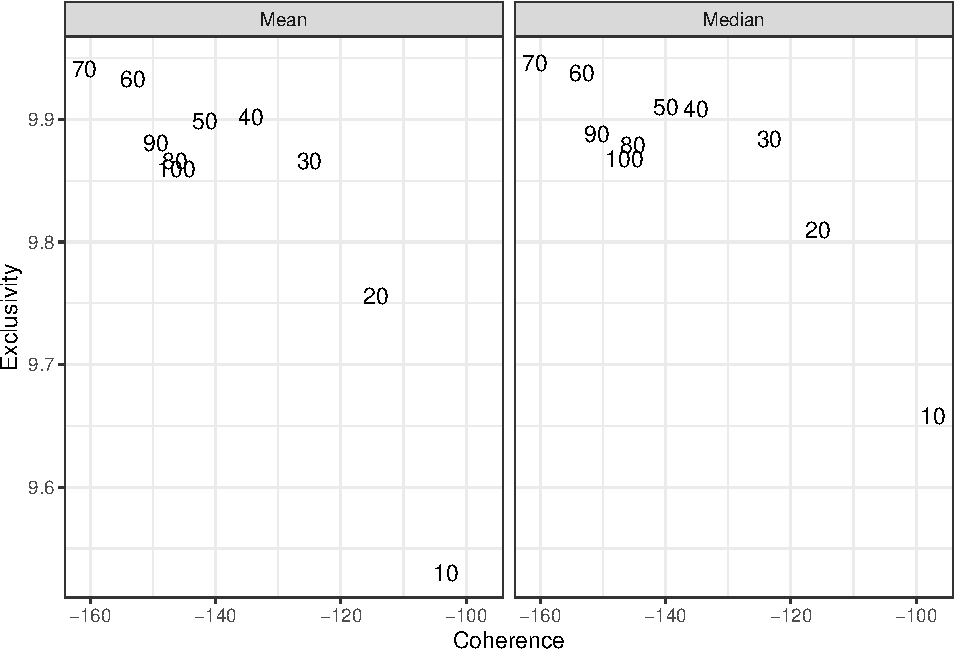
\includegraphics{workshop_topicmodels_files/figure-latex/model-compare-1.pdf}

\begin{Shaded}
\begin{Highlighting}[]
\CommentTok{# Exklusivität und Semantische Kohärenz von k = 40, 50}
\NormalTok{model_eval }\OperatorTok\StringTok{ }
\StringTok{  }\KeywordTok{filter}\NormalTok{(K }\OperatorTok\StringTok{ }\KeywordTok{c}\NormalTok{(}\DecValTok{40}\NormalTok{, }\DecValTok{50}\NormalTok{)) }\OperatorTok\StringTok{ }
\StringTok{  }\KeywordTok{select}\NormalTok{(K, }\DataTypeTok{Exclusivity =}\NormalTok{ exclusivity, }\DataTypeTok{Coherence =}\NormalTok{ semantic_coherence) }\OperatorTok\StringTok{ }
\StringTok{  }\KeywordTok{unnest}\NormalTok{(}\KeywordTok{c}\NormalTok{(Exclusivity, Coherence)) }\OperatorTok\StringTok{ }
\StringTok{  }\KeywordTok{ggplot}\NormalTok{(}\KeywordTok{aes}\NormalTok{(Coherence, Exclusivity, }\DataTypeTok{color =} \KeywordTok{factor}\NormalTok{(K))) }\OperatorTok{+}\StringTok{ }\KeywordTok{geom_point}\NormalTok{()}
\end{Highlighting}
\end{Shaded}

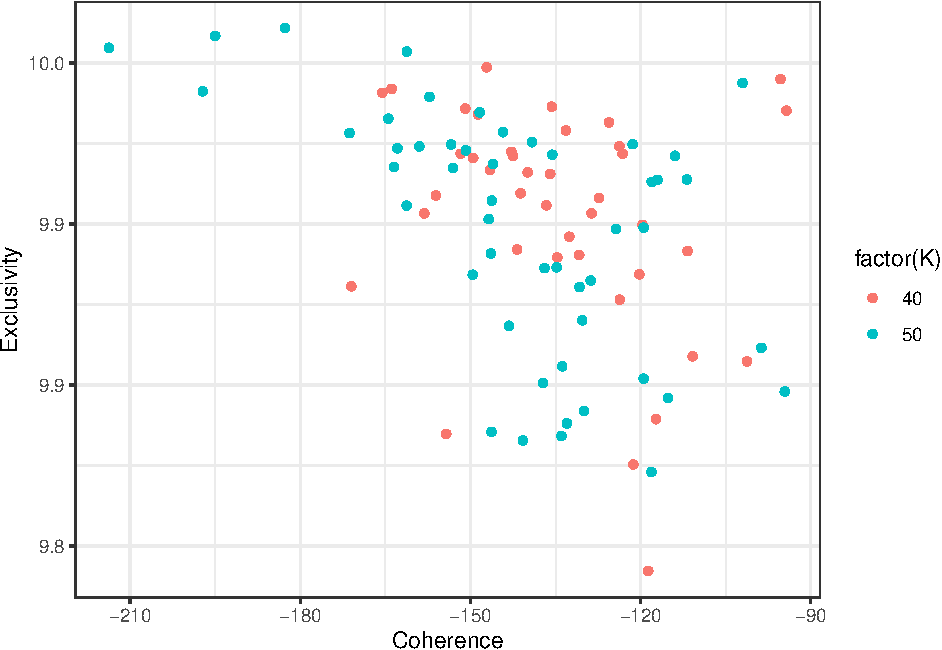
\includegraphics{workshop_topicmodels_files/figure-latex/model-compare-2.pdf}

\begin{Shaded}
\begin{Highlighting}[]
\CommentTok{# Held-out-likelihood und multinomiale Residuen}
\NormalTok{model_eval }\OperatorTok\StringTok{ }
\StringTok{  }\KeywordTok{select}\NormalTok{(K, }\StringTok{`}\DataTypeTok{Held-out likelihood (higher is better)}\StringTok{`}\NormalTok{ =}\StringTok{ }\NormalTok{held_out_likelihood, }\StringTok{`}\DataTypeTok{Multinomial dispersion of residuals (lower is better)}\StringTok{`}\NormalTok{ =}\StringTok{ }\NormalTok{residuals) }\OperatorTok\StringTok{ }
\StringTok{  }\KeywordTok{gather}\NormalTok{(measure, value, }\OperatorTok{-}\NormalTok{K) }\OperatorTok\StringTok{ }
\StringTok{  }\KeywordTok{ggplot}\NormalTok{(}\KeywordTok{aes}\NormalTok{(K, value, }\DataTypeTok{label =}\NormalTok{ K)) }\OperatorTok{+}\StringTok{ }\KeywordTok{geom_line}\NormalTok{() }\OperatorTok{+}\StringTok{ }\KeywordTok{geom_text}\NormalTok{() }\OperatorTok{+}\StringTok{ }\KeywordTok{facet_wrap}\NormalTok{(}\StringTok{"measure"}\NormalTok{, }\DataTypeTok{scales =} \StringTok{"free_y"}\NormalTok{, }\DataTypeTok{ncol =} \DecValTok{1}\NormalTok{) }\OperatorTok{+}\StringTok{ }\KeywordTok{labs}\NormalTok{(}\DataTypeTok{x =} \StringTok{"Number of topics (K)"}\NormalTok{, }\DataTypeTok{y =} \OtherTok{NULL}\NormalTok{)}
\end{Highlighting}
\end{Shaded}

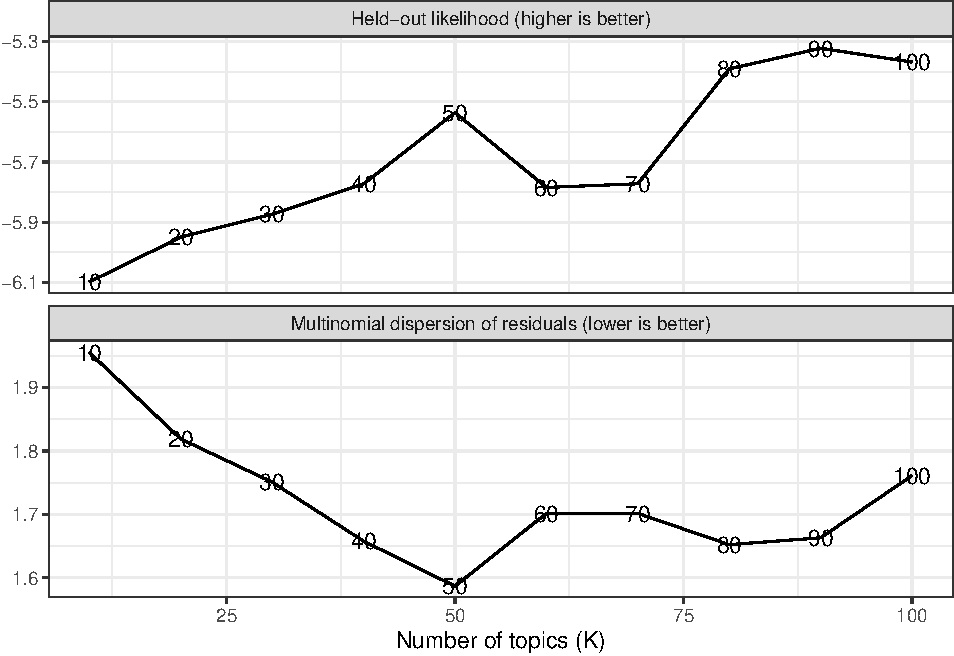
\includegraphics{workshop_topicmodels_files/figure-latex/model-compare-3.pdf}

\begin{Shaded}
\begin{Highlighting}[]
\CommentTok{# Speichern der Modelle mit 30 und 40 Topics für qualitative Analyse}
\CommentTok{# Benennung und Datenstruktur für stminsights}
\NormalTok{out =}\StringTok{ }\NormalTok{impf_stm}
\NormalTok{m30 =}\StringTok{ }\NormalTok{many_models}\OperatorTok{$}\NormalTok{topic_model[[}\DecValTok{3}\NormalTok{]]}
\NormalTok{m40 =}\StringTok{ }\NormalTok{many_models}\OperatorTok{$}\NormalTok{topic_model[[}\DecValTok{4}\NormalTok{]]}
\NormalTok{m60 =}\StringTok{ }\NormalTok{many_models}\OperatorTok{$}\NormalTok{topic_model[[}\DecValTok{6}\NormalTok{]]}
\CommentTok{# save(out, m30, m40, m60, file = "R/data/models30_40_60.rdata")}
\end{Highlighting}
\end{Shaded}

\begin{itemize}
\tightlist
\item
  Wir betrachten zuerst die \emph{semantische Kohärenz} und die \emph{Exklusivität} der Topics in den Modellen. Beide Metriken sind Eigenschaften der einzelnen Themen. In der ersten Grafik sind daher der Mittelwerte und die Mediane aller Themen in einem Modell dargestellt. Die absoluten Werte beider Metriken haben keine substantielle Bedeutung. Von Interesse ist der Vergleich der Modelle. Je höher die Exklusivität, desto geringer ist die Wahrscheinlichkeit, dass die typischsten Terme eines Topics in anderen Topics vorkommen \citep{robertsStructuralTopicModels2014}. Je höher die semantische Kohärenz, desto wahrscheinlicher kommen die typischsten Wörter eines Topics gemeinsam in einem Dokument mit diesem Topic vor \citep{davidmimnoOptimizingSemanticCoherence2011}. Zwischen den beiden Metriken besteht in der Regel ein negativer Zusammenhang. Daher ist es notwendig, eine Balance zwischen beiden zu finden.

  \begin{itemize}
  \tightlist
  \item
    Im vorliegenden Beispiel können wir zuerst die Modelle mit \(k \ge 80\) ausschließen. Obwohl sie mehr Topics benötigen, sind ihre Topics im Mittel weniger exklusiv und weniger kohärent als die Topics der Modelle \(k = 60\) oder \(k = 70\). Eine Erklärung dafür kann sein, irgendwann zwischen dem 70. und dem 80. Topic keine substantiell neuen Aspekte mehr im Korpus zu finden sind. Die neuen Topics sind dann redundant zu schon bestehenden Topics.
  \item
    Ebenso können wir für die meisten Zwecke die Modelle mit \(k \le 20\) vernachlässigen, da die mittlere Exklusivität ihrer Topics wesentlich geringer ist als die der übrigen Modelle. Das Modell mit \(k = 20\) könnte vielleicht infrage kommen, wenn wir Sparsamkeit sehr hoch gewichten, also den Korpus durch möglichst wenige Topics beschreiben wollen.
  \item
    Schließlich ist das Modell mit \(k = 50\) nicht besonders attraktiv. Die Topics sind im Mittel nur weniger kohärent, aber nicht exklusiver, als die Topics des Modells mit \(k = 40\). Der Detailvergleich der beiden Modelle in der nächsten Abbildung, in der jedes Topic mit einem Punkt dargestellt ist, zeigt, dass dies vor allem auf vier Topics zurück geht, die weniger kohärent sind, ohne eine besonders gute Exklusivität aufzuweisen.
  \item
    Gegeben der Metriken \emph{semantische Kohärenz} und \emph{Exklusivität} spricht einiges dafür, entweder Modelle mit ca. 60-70 Topics oder Modelle mit 30-40 Topics weiter zu verfolgen.
  \end{itemize}
\item
  Die \emph{held-out likelihood} und die \emph{Dispersion der multinomialen Residuen} sind zwei Metriken, die die Abweichung des Modells von den Daten quantifizieren. Auch sie sind wieder im relativen Modellvergleich zu interpretieren. Die held-out likelihood gibt Auskunft darüber, wie gut das Vorkommen von Wörter in einem Dokument, das nicht zum Schätzen des Modells genutzt wurde, vorhergesagt werden kann. Mit der Dispersion der multinomialen Residuen wird die Abweichung der durch das Modell vorhergesagten von den beobachteten Wörtern in den Dokumenten auf Basis des gesamten Datensatzes quantifiziert. Ein Wert von 1 wäre ideal, wird in angewandten Beispielen mit echten Texten aber kaum erreicht. Beide Metriken sind eng verwandt und legen in der Regel ähnliche Entscheidungen nahe.

  \begin{itemize}
  \tightlist
  \item
    Das Modell mit \(k = 50\) ist nach beiden Metriken gut geeignet.
  \item
    Nach der held-out likelihood sind die Modelle mit \(k \ge 80\) noch etwas besser - diese haben sich aber in der semantischer Kohärenz und Exklusivität nicht sonderlich gut bewährt.
  \item
    Die nach semantischer Kohärenz und Exklusivität besten Modelle liegen nach diesen beiden Metriken etwa gleich auf.
  \end{itemize}
\item
  Die Befunde sind auch für die didaktischen Zwecke dieses Workshops gut geeignet. Es wird klar, dass die Modellwahl sich nicht einfach automatisieren lässt. Die quantitativen Kriterien helfen und lediglich, den Raum möglicher Modelle einzuschränken.

  \begin{itemize}
  \tightlist
  \item
    Für mich kommen auf Basis der berichteten Metriken Modelle mit zwischen 30 und 70 Topics infrage.
  \item
    Wenn man an einer besonders sparsamen Lösung interessiert ist, könnte man auch \(k = 20\) in Erwägung ziehen.
  \item
    Wenn man besonders detailliertere Lösungen sucht, sind auch die Modelle mit \(k \ge 80\) nicht ausgeschlossen. Hier müsste man dann die Differenzierungen zwischen den Topics in der Tiefe untersuchen und klarstellen.
  \end{itemize}
\item
  Im nächsten Schritt vergleichen wir die Modelle mit 30 und mit 60 Topics, um zu verstehen, welche Konsequenzen es für die inhaltliche Interpretation hat, ein eher sparsames oder ein eher detailliertes Modell zu wählen. Nach dieser Entscheidung können wir dann weiter überlegen, welches der eher sparsamen bzw. detaillierten Modelle für unser Forschungsinteresse besser geeignet ist.
\end{itemize}

\hypertarget{qualitativer-vergleich-der-modelle-mit-30-und-60-topics}{%
\subsection{Qualitativer Vergleich der Modelle mit 30 und 60 Topics}\label{qualitativer-vergleich-der-modelle-mit-30-und-60-topics}}

\begin{itemize}
\tightlist
\item
  Um die Ergebnisse eines Topic Model interpretieren zu können, müssen wir zuerst verstehen, wie das Ergebnis eines Topic Models aussieht. Es enthält im wesentlichen zwei zweidimensionale Vektoren von Koeffizienten.

  \begin{itemize}
  \tightlist
  \item
    beta: Für jedes Topic die Wahrscheinlichkeit, dass ein Dokument, in dem das Feature vorkommt, das Topic hat. Jedes Topic erhält für jedes Feature einen beta-Koeffizienten zwischen 0 und 1, die zusammen 1 ergeben.
  \item
    theta bzw. gamma (uneinheitlich benannt): Für jedes Dokument die Wahrscheinlichkeit, dass das Dokument das Topic enthält. Jedes Dokument erhält für jedes Topic einen theta- bzw. gamma-Koeffizienten zwischen 0 und 1, die zusammen 1 ergeben.
  \end{itemize}
\item
  Um die Bedeutung der Topics zu interpretieren, betrachten wir daher zwei Modell-Outputs.

  \begin{itemize}
  \tightlist
  \item
    Die Features, die am typischsten für Dokumente mit einem Topic sind, also die höchsten beta-Koeffizienten (ggf. nach Korrekturen für die Verteilung der Features im gesamten Korpus).
  \item
    Die Dokumente, die mit der größten Wahrscheinlichkeit ein Thema enthalten (manchmal auch interpretiert als zum größten Anteil aus einem Thema bestehen), also die Dokumente mit den höchsten gamma- bzw. theta-Koeffizienten.
  \end{itemize}
\item
  Zur qualitativen Interpretation der Modelle anhand dieser Outputs kann ich das Paket \texttt{\{stminsights\}} empfehlen --- vor allem denjenigen, die lieber mit einer intuitiven grafischen Benutzeroberfläche als direkt mit \emph{R} arbeiten. Aber auch ich selbst schätze das Tool für einen schnellen Überblick über mehrere Modelle.
\item
  Leider ist es zurzeit nicht einfach, \texttt{\{stminsights\}} direkt zum Laufen zu bringen, da einige Pakete, auf denen es aufbaut, Bugs bzw. Kompabilitätsprobleme haben. Eine Anleitung, wie das Paket zurzeit installiert werden kann, gibt es hier:
\end{itemize}

\begin{quote}
Important note: The shiny app for the CRAN release of stminsights does currently not work properly due to bugs introduced by recent changes in the Shiny package {[}\ldots{]}. Please use the Github version of stminsights for now. This will require the development version of Shiny which can be installed by running devtools::install\_github(`rstudio/shiny').
\end{quote}

\begin{quote}
You can download and install the latest development version of stminsights by running devtools::install\_github(`cschwem2er/stminsights') --- \url{https://github.com/cschwem2er/stminsights}
\end{quote}

\begin{itemize}
\tightlist
\item
  Zur Vorbereitung der Analyse mit \texttt{\{stminsights\}} müssen die Objekte der geschätzten Modelle (hier: \texttt{m30}, \texttt{m40} {[}brauchen wir etwas später{]} und \texttt{m60}) und die Daten, die zur Modellschätzung verwendet wurden (hier: \texttt{out\ =\ ìmpf\_stm}), als \texttt{.rdata} Datei gespeichert werden. Dabei muss das Daten-Objekt \emph{unbedingt} den Namen \texttt{out} haben. Damit der Text der Dokumente in \texttt{\{stminsights\}} angezeigt werden kann, muss dieser zusätzlich als Variable in den Meta-Daten enthalten sein (siehe Abschnitt zur Datenaufbereitung).
\item
  Durch das ausführen der Funktion \texttt{run\_stminsights()} wird eine grafische Benutzeroberfläche im Browser gestartet, mit dem die qualitative Analyse durchgeführt wird. Eine Beschreibung der Oberfläche findet ihr als Video im LMS {[}kommt nach Fertigstellen des Textmaterials{]}.
\end{itemize}

\begin{Shaded}
\begin{Highlighting}[]
\KeywordTok{run_stminsights}\NormalTok{()}
\end{Highlighting}
\end{Shaded}

\begin{itemize}
\tightlist
\item
  Wer die Interpretation der Topics lieber in R durchführt, kann z.B. den folgenden Code verwenden und anpassen.

  \begin{itemize}
  \tightlist
  \item
    Wir sammeln zuerst die 20 typischsten Texte für jedes Topic in einem Datensatz. Dabei bereiten wir die Texte auch für eine Ausgabe in der Konsole vor. Der Parameter ``gamma'' oder ``theta'' (uneinheitlich benannt, aber derselbe Parameter) kann mit \texttt{tidytext::tidy()} extrahiert werden. Dann werden die Texte aus den Ursprungsdaten zugespielt.
  \item
    Mit \texttt{stm::labelTopics()} können wird die typischsten Features für ein Topic anzeigen. \texttt{n} bestimmt die Zahl der Features, \texttt{topics} das Topic, das wir gerade beschreiben möchten. Es werden die typischsten Features nach vier verschiedenen Kriterien ausgegeben (Diese werden auch in \texttt{\{stminsights\}} angezeigt):

    \begin{itemize}
    \tightlist
    \item
      \emph{Highest Prob} zeigt die Features, die mit der größten Wahrscheinlichkeit in Dokumenten mit einem Topic vorkommen (= Features mit den höchsten beta-Koeffizienten für das Topic). Dabei wird die Gesamthäufigkeit der Features im Korpus \emph{nicht} berücksichtigt. Wörter, die allgemein sehr häufig vorkommen, sind nach dieser Metrik typisch für verschiedene Topics. Die anderen drei Metriken versuchen, diese Schwäche auf verschiedene Art und Weise zu korrigieren.
    \item
      \emph{FREX} steht für \emph{most frequent and exclusive} Features. Hier werden die Features aufgelistet, die möglichst typisch für ein Dokument mit einem Topic, aber möglichst nicht sehr typisch für Dokumente mit anderen Topics sind. Siehe \texttt{?calcfrex} für technische Details.
    \item
      Die \emph{Lift}-Metrik setzt die Wahrscheinlichkeit, dass ein Feature in einem Dokument mit einem Topic vorkommt, zur Wahrscheinlichkeit, dass ein Feature in einem beliebigen Dokument vorkommt, ins Verhältnis. Siehe \texttt{?calclift} für technische Details.
    \item
      \emph{Score} gewichtet für die Wahrscheinlichkeit, mit der ein Feature in Dokumenten mit einem anderen Topics vorkommt. Siehe \texttt{?calcscore} für technische Details.
    \end{itemize}
  \item
    Mit den Auszügen aus dem Datensatz typischer Dokumente (gefiltert nach Topic) können wir diese Features zudem im Kontext der gesamten Texte sehen.
  \item
    Im abschließenden Datensatz \texttt{topic\_labels} halten wir für jedes Topic ein aussagekräftiges, möglichst kurzes Label fest, das wir jetzt zur eigenen Übersicht und später auch zur Ergebnisdarstellung verwenden. Zusätzlich empfehle ich, eine kurze Zusammenfassung für jedes Topic auf einem Medium eigener Wahl (präferierte analoger oder digitaler Notizzettel) festzuhalten.
  \end{itemize}
\end{itemize}

\begin{Shaded}
\begin{Highlighting}[]
\CommentTok{# Laden der Modelle}
\KeywordTok{load}\NormalTok{(}\StringTok{"R/data/models30_40_60.rdata"}\NormalTok{)}

\CommentTok{# Beispiel für das Modell mit k = 30}
\CommentTok{# Erstellen eines Datensatzes mit den typischsten Dokumenten}
\NormalTok{top_docs =}\StringTok{ }\KeywordTok{tidy}\NormalTok{(m30, }\StringTok{"gamma"}\NormalTok{) }\OperatorTok\StringTok{ }
\StringTok{  }\KeywordTok{arrange}\NormalTok{(}\KeywordTok{desc}\NormalTok{(gamma)) }\OperatorTok\StringTok{ }
\StringTok{  }\KeywordTok{group_by}\NormalTok{(topic) }\OperatorTok\StringTok{ }
\StringTok{  }\KeywordTok{slice}\NormalTok{(}\DecValTok{1}\OperatorTok{:}\DecValTok{20}\NormalTok{) }\OperatorTok\StringTok{ }
\StringTok{  }\KeywordTok{mutate}\NormalTok{(}\DataTypeTok{rank =} \DecValTok{1}\OperatorTok{:}\DecValTok{20}\NormalTok{) }\OperatorTok\StringTok{ }
\StringTok{  }\KeywordTok{left_join}\NormalTok{(}\KeywordTok{mutate}\NormalTok{(}\KeywordTok{select}\NormalTok{(out}\OperatorTok{$}\NormalTok{meta, txt), }\DataTypeTok{document =} \DecValTok{1}\OperatorTok{:}\KeywordTok{n}\NormalTok{())) }\OperatorTok\StringTok{ }
\StringTok{  }\KeywordTok{mutate}\NormalTok{(}\DataTypeTok{out =} \KeywordTok{paste0}\NormalTok{(}\KeywordTok{round}\NormalTok{(gamma, }\DecValTok{2}\NormalTok{), }\StringTok{": "}\NormalTok{, txt))}

\CommentTok{# Ausgabe der typischen Feature für ein Topic (hier Topic 1)}
\NormalTok{m30 }\OperatorTok\StringTok{ }
\StringTok{  }\KeywordTok{labelTopics}\NormalTok{(}\DataTypeTok{n =} \DecValTok{10}\NormalTok{, }\DataTypeTok{topics =} \DecValTok{1}\NormalTok{)}
\end{Highlighting}
\end{Shaded}

\begin{verbatim}
## Topic 1 Top Words:
##       Highest Prob: 2, 3, 1, monate, erst, monaten, 4, 6, alt, 5 
##       FREX: 3, 2, monate, monaten, 6, 4, 1, monat, +, 5 
##       Lift: österreich, zecken, monat, fach, 3, 2, monate, 6, +, monaten 
##       Score: österreich, 2, 3, monate, 1, monaten, 4, alt, 6, +
\end{verbatim}

\begin{Shaded}
\begin{Highlighting}[]
\CommentTok{# Ausgabe der typischen Texte für ein Topic (hier Topic 1)}
\NormalTok{top_docs }\OperatorTok
\StringTok{  }\KeywordTok{filter}\NormalTok{(topic }\OperatorTok{==}\StringTok{ }\DecValTok{1}\NormalTok{) }\OperatorTok\StringTok{ }
\StringTok{  }\KeywordTok{filter}\NormalTok{(rank }\OperatorTok\StringTok{ }\DecValTok{1}\OperatorTok{:}\DecValTok{10}\NormalTok{) }\OperatorTok\StringTok{ }
\StringTok{  }\NormalTok{.}\OperatorTok{$}\NormalTok{out }\OperatorTok\StringTok{ }
\StringTok{  }\KeywordTok{str_squish}\NormalTok{() }\OperatorTok\StringTok{ }
\StringTok{  }\KeywordTok{cat}\NormalTok{(}\DataTypeTok{sep =} \StringTok{"}\CharTok{\textbackslash{}n\textbackslash{}n}\StringTok{"}\NormalTok{)}
\end{Highlighting}
\end{Shaded}

\begin{verbatim}
## 0.62: da fängt der 12 lebensmonat an, ein Jahr alt ist dein Baby dann erst mit vollendetem 12. Lebensmonat.... meine Tochter wird jetzt am 24.07 12 Monate alt, und am 24.08 wird sie 1 Jahr....da ist also der 12 lebensmonat vollendet :)
## 
## 0.59: Man spricht erst sobald der Monat vollendet ist vom z.B. 12. Monat. Deine Tochter ist also einen Monat vor ihrem 1. Geburtstag ELF Monate alt und nicht 12... Klar, sie befindet sich ab dem 24.07. im zwölften Lebensmonat, ist aber noch keine 12 Monate alt, sondern 11. Kann etwas verwirrend sein, ich weiß... Denn sie ist am Tag ihrer Geburt ja auch nicht einen Monat alt... Sondern erst einen Monat nach ihrer Geburt Ich bin aktuell 30 Jahre alt und befinde mich somit in meinem 31. Lebensjahr. So wird das immer gerechnet :)
## 
## 0.59: In Österreich wird im 3., 5. und 12. Monat geimpft. Ich bin auf einer anderen Seite auch fündig geworden. Dieses Schema nennt sich 2+1. Das in Deutschland von der Stiko empfohlene Schema nennt sich 3+1. Beide Schemata werden wohl in Deutschland als Grundimmunisierung anerkannt, da das Schema 2+1 einen ähnlichen bzw. gleichen Effekt hat wie 3+1. Die Stiko empfiehlt halt das 3+1 Schema.
## 
## 0.53: so mein ich ja :) sie befindet sich ab dem Tag ihrer Geburt ja im erst Lebensmonat und nicht im nullsten Lebensmonat :D und ab dem 24.07 ist sie im 12. Öebensmonat.... wenn mich jemand Frägt wie alt sie ist sag ich auch nich 12 Monate alt sonder sie wird Ende August 1 Jahr alt...aber prinzipiell, so wird es auch bei Urbia angezeigt ist sie ab 24.07 im 12 lebensmonat....und wenn der vollendet ist, wird sie 1... :)
## 
## 0.51: Wir mussten 2 Monate auf den Termin beim Kardiologen warten. Hatten den Termin dann als er jetzt 6 Monate alt war. Das Herzgeräusch sind 2 Sehnenfäden, aber er hat auch ein Mini Loch. Wir müssen erst wieder zur Kontrolle, wenn er 3 Jahre ist.
## 
## 0.5: Korrektur: Bei der 2+1 Impfung sind ca 84% nach der 2 . Impfung immun. Bei der 3+1 Impfung sind ca 95 % nach der 3. Impfung immun. Und die ersten beiden bzw. 3 Impfungen werden ja in einen Zeitraum von 2 Monaten verabreicht. Also durchaus noch abzuwarten, wenn du dir da Sorgen machst.
## 
## 0.47: hallo rebecca es gibt auch "Mittelwege", zB das 2+1-Schema. Man beginnt erst mit 3 Monaten und spart sich eine Impfdosis. (Normalerweise ist ja 3 x innerhalb des 1. Lebensjahres und 1 x zur Auffrischung). Die Immunantwort ist am Ende wohl identisch, das Risiko besteht darin, dass man eben 1 Monat später beginnt und damit der Impfschutz 1 monat später beginnt. Wobei das größte Risiko hier der Keuchhusten ist. Das 2+1-Schema ist zB in Österreich Standard.
## 
## 0.47: Unter 2 Jahren muss 2x geimpft werden. Mein Sohn ist 6 Monate. Wird am Freitag geimpft und dann in 2 Monaten wieder. Die Dritte erfolgt wenn er 2 Jahre alt ist oder 3 Jahre. Du musst alle 3 Impfungen bezahlen jeweils 120 Euro oder ein bisschen mehr. Die AOK Niedersachsen wird diese 3 Impfungen jeweils mit 80% mir erstatten. Die AOK Sachsen anscheinend alle 3 zu 100%.
## 
## 0.44: Dann wär er aber 1 Monat vor Geburtstag 12 Monate : Wenn du die Wochen zählst darfst du halt nicht 4 Wochen mit 1 Monat gleich setzen.
## 
## 0.43: Darf ich über die Fragestellung hinaus fragen, wie genau der Ablauf dann genau ist. Befasse mich in den ersten Zügen mit dem Thema Impfen. Es wird also in den ersten 12 Monaten 2x 5fach geimpft und dann 1x bis zum 24 Monat? Kann man das system 2+1 auch auf 6fach-impfung übertragen? Und auf +pneumokokken?
\end{verbatim}

\begin{Shaded}
\begin{Highlighting}[]
\CommentTok{# Datensatz für Topic Labels}
\CommentTok{# Bis Topic 30 weiterführen}
\NormalTok{m30_topic_labels =}\StringTok{ }\KeywordTok{tribble}\NormalTok{(}
  \OperatorTok{~}\NormalTok{topic, }\OperatorTok{~}\NormalTok{label,}
  \DecValTok{1}\NormalTok{,      }\StringTok{"Alter von Babies"}\NormalTok{,}
  \DecValTok{2}\NormalTok{,      }\StringTok{"label B"}\NormalTok{,}
  \DecValTok{3}\NormalTok{,      }\StringTok{"label C"}
\NormalTok{)}
\end{Highlighting}
\end{Shaded}

\begin{itemize}
\tightlist
\item
  Die Labels aus meiner vorläufigen Interpretation finden sich in \texttt{R/topic\_labels.R} (hier nicht dargestellt).

  \begin{itemize}
  \tightlist
  \item
    Die meisten Topics des Modells mit \(k = 30\) erwiesen sich als gut interpretierbar. An der einen oder anderen Stelle schien es aber so, als seien mehrere Aspekte der Impfdiskussionen in einem Topic vermischt. Dies könnte auf eine etwas größere Topic-Anzahl hindeuten.
  \item
    Die Interpretation der Topics des Modells mit \(k = 60\) fiel mir wesentlich schwerer. Die typischen Features vieler Topics waren zwar exklusiv für das jeweilige Topic, waren aber nicht direkt als ein Aspekt Diskussionen zum Thema impfen zu interpretieren. Häufig scheinen hier auch Terme, die z.B. aus Gründen der Formulierung häufiger zusammen auftauchen, ein Topic zu bilden.
  \item
    Der qualitative Vergleich der beiden Modelle legt für mich nahe, dass ein nützliches Modell eher in der Region etwas über \(k = 30\) zu finden ist als bei \(k = 60\). Der Grund dafür ist, dass ich meist Modelle mit möglichst vielen interpretierbare Topics bevorzuge. Wenn --- wie in diesem Beispiel --- die Dokumente bereits so ausgewählt wurden, dass die meisten Dokumente prinzipiell für das Forschungsinteresse relevant sind, halte ich es für sinnvoll, über einen möglichst großen Anteil der inhaltlichen Varianz in diesen Dokumenten etwas auszusagen. Topics, die aus der Analyse ausgeschlossen werden müssen, helfen nicht dabei, die Inhalte der Dokumente zu beschreiben und zu verstehen.
  \item
    Beachtet aber, dass das nicht die einzige sinnvolle Vorgehensweise ist. Topic Models enthalten fast immer einige Topics, die sich nicht mit Blick auf das Forschungsinteresse interpretieren lassen \citep{maierApplyingLDATopic2018}. Diese werden dann häufig von den weiteren Analysen ausgeschlossen. Die Analysen der interpretierbaren Topics sind davon nicht weiter beeinträchtigt, solange die nicht interpretierbaren Topics keine relevanten Informationen aus den interpretierbaren Topic entfernen. Wir könnten nach dieser Logik also auch das Modell mit \(k = 60\) zum Ausgangspunkt der Suche nach dem nützlichsten Modell machen und viele Topics ausschließen. Die Argumentation wäre dann, dass die verbliebenen Topics besonders klar herausstechen, da die nicht relevanten Charakteristika der Dokumente in den nicht relevanten Topics stecken.
  \item
    Aus diesem Grund habe ich als nächsten Schritt das Modell mit \(k = 40\) zum Vergleich herangezogen. Dabei bestätigt sich nach meiner Wahrnehmung die Vermutung, dass (etwas) mehr als 30 Topics eine geeignete Wahl sein könnten.
  \end{itemize}
\end{itemize}

\hypertarget{schuxe4tzen-und-vergleich-von-weiteren-modellen-zwischen-k-30-und-k-40}{%
\subsection{\texorpdfstring{Schätzen und Vergleich von weiteren Modellen zwischen \(k = 30\) und \(k = 40\)}{Schätzen und Vergleich von weiteren Modellen zwischen k = 30 und k = 40}}\label{schuxe4tzen-und-vergleich-von-weiteren-modellen-zwischen-k-30-und-k-40}}

\begin{itemize}
\tightlist
\item
  Die Spezifikation und er quantitative Vergleich erfolgt nach demselben Prinzip wie zuvor. Der Code ist daher hier nicht dargestellt, kann aber in \texttt{R/model\_compare2.R} gefunden werden. Wir vergleichen alle Modelle zwischen \(k = 30\) und \(k = 40\).
\end{itemize}

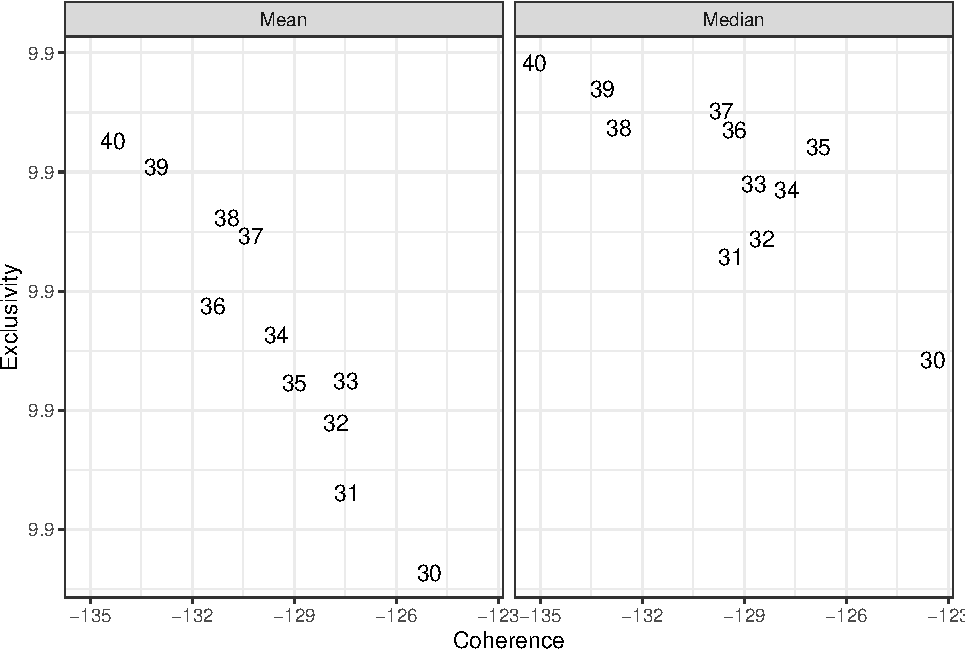
\includegraphics{workshop_topicmodels_files/figure-latex/model-compare2-1.pdf} 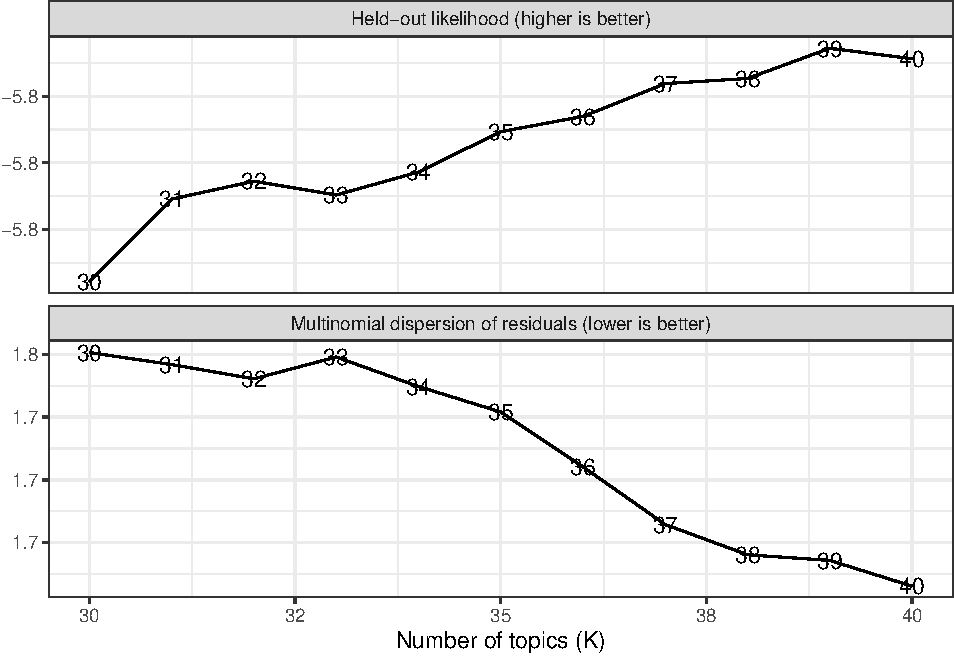
\includegraphics{workshop_topicmodels_files/figure-latex/model-compare2-2.pdf}

\begin{itemize}
\tightlist
\item
  Ein Blick auf die Skalierung der Achsen zeigt, dass die Modelle sich untereinander nur wenig unterscheiden. Die quantitativen Metriken helfen uns bei der Entscheidung zwischen diesen Modellen nicht weiter.
\item
  Es folgt ein recht aufwändiger qualitativer Prozess, in dem wir entscheiden, ob die zusätzlichen Themen die Beschreibung der Dokumentinhalte substantiell verbessern.
\end{itemize}

  \bibliography{book.bib}

\end{document}
